\documentclass[openany]{book}
% openany: keine leere Seite vor Kapitel

% \usepackage[utf8]{inputenc}
\usepackage{polyglossia}
\usepackage[a4paper, landscape, margin=2cm, twoside, bindingoffset=1cm]{geometry}
\usepackage{multicol}
\usepackage[labelformat=simple]{subfig}
\usepackage{graphicx}
\usepackage{wrapfig}
% \usepackage{showframe}
\usepackage{lipsum}
\usepackage{verbatim}
\usepackage{eso-pic}
\usepackage{fancyhdr}
\usepackage{tikz}
\usepackage[newparttoc]{titlesec}
\usepackage{titletoc}
\usepackage{xfrac}
\usepackage{pdfpages}
\usepackage{forloop}
\usepackage[export]{adjustbox}
\usepackage{caption}
\usepackage{csquotes}
\usepackage{threeparttable}
\usepackage{longtable}
\usepackage{floatpag}
\usepackage{enumitem}

\setdefaultlanguage[variant=swiss]{german}

\makeatletter
% change title size
\patchcmd{\@maketitle}{\normalsize}{\HUGE}{}{}
% change author size
\patchcmd{\@setauthors}{\MakeUppercase {\authors }}{\MakeUppercase{\Large\authors}}{}{}
% change section title size
\patchcmd{\section}{\normalfont}{\normalfont\Large}{}{}
\makeatother

% TOC formatting
\setcounter{tocdepth}{0} % Show only \part and \chapter in tableofcontents
\makeatletter
\let\latexl@part\l@part
\def\l@part#1#2{\begingroup\let\numberline\@gobble\latexl@part{#1}{#2}\endgroup}
\makeatother

\makeatletter
\let\latexl@chapter\l@chapter
\def\l@chapter#1#2{\begingroup\let\numberline\@gobble\latexl@chapter{#1}{#2}\endgroup}
\makeatother

\titleformat{\part}{\normalfont\Huge\bfseries}{}{0em}{}
\titleformat{\chapter}{\normalfont\huge\bfseries}{}{0em}{}
\titleformat{\section}{\normalfont\Large\bfseries}{}{0em}{}
\titleformat{\subsection}{\normalfont\large\bfseries}{}{0em}{}
\titleformat{\subsubsection}{\normalfont\normalsize\bfseries}{}{0em}{}
\titleformat{\paragraph}[runin]{\normalfont\normalsize\bfseries}{}{0em}{}
\titleformat{\subparagraph}[runin]{\normalfont\normalsize\bfseries}{0}{0em}{}

\titlespacing{\part}{0em}{0em}{0em}
\titlespacing{\chapter}{0em}{0em}{0em}


\setlist[itemize]{leftmargin=0cm}

% redefine plain style (used by first pages of chapters)
\fancypagestyle{plain}{
    \lhead{}
    \fancyhead{}
    \fancyfoot{}
    \renewcommand{\headrulewidth}{0pt}
}

\fancyhf{}
\fancyhead[RO]{\leftmark{}}
\fancyhead[LE]{\leftmark{}}
\fancyfoot[RO]{\thepage}
\fancyfoot[LE]{\thepage}
\pagestyle{fancy}
\floatpagestyle{fancy} % required for float-only pages

\renewcommand{\headrulewidth}{0pt}
\renewcommand{\chaptermark}[1]{\markboth{#1}{}}
% \renewcommand{\chaptermark}[1]{}
\renewcommand{\sectionmark}[1]{\markboth{#1}{}}
% \renewcommand{\sectionmark}[1]{}
\renewcommand{\subsectionmark}[1]{} % ignore subsections in header
\AddToHook{cmd/section/before}{\clearpage} % new page on each section

\renewcommand{\thesubfigure}{\relax}  % Do nothing for the counter »subfigure«


\setlength\columnsep{1cm} %distance between multicolumn columns
\captionsetup{font=small, labelformat=empty} % Bildtitel ohne Kapitelangabe
\captionsetup[subfigure]{justification=justified,singlelinecheck=false}

\newcommand{\groupphoto}[5]{
    {
            \captionsetup{singlelinecheck=false} % left aligned
            \begin{figure}[!htbp]
                \thisfloatpagestyle{empty}
                \centering
                \begin{measuredfigure}
                    \includegraphics[width=#1\textwidth,height=#2\textheight, keepaspectratio]{#3}
                \end{measuredfigure}
                \caption{#4}
                \label{#5}
            \end{figure}
        }
}

\newcommand{\portrait}[3][0.8]{
    {
            \captionsetup{singlelinecheck=false} % left aligned
            \begin{figure}[!htbp]
                \def\theight{#1}
                \begin{measuredfigure}
                    \includegraphics[width=0.93\textwidth, height=\theight\textheight, keepaspectratio]{#2}
                    \caption{#3}
                \end{measuredfigure}
            \end{figure}
        }
}
\newcommand{\ConcertProg}[2][0.8]{{
            \begin{figure}[!htbp]
                \centering
                \includegraphics[height=#1\textheight,keepaspectratio]{#2}%
            \end{figure}
        }}

\newcommand{\ConcertProgsTwoVertical}[3][0.485]{{
            \begin{figure}[!htbp]
                \centering
                \subfloat{%
                    \includegraphics[height=#1\textheight,keepaspectratio]{#2}%
                }\\
                \subfloat{%
                    \includegraphics[height=#1\textheight,keepaspectratio]{#3}%
                }
            \end{figure}
        }}

\newcommand{\ConcertProgsTwoHorizontal}[3][0.85]{{
            \begin{figure}[!htbp]
                \centering
                \subfloat{%
                    \includegraphics[height=#1\textheight,keepaspectratio]{#2}%
                }\hfil
                \subfloat{%
                    \includegraphics[height=#1\textheight,keepaspectratio]{#3}%
                }
            \end{figure}
        }}

\newcommand{\ConcertProgsFourOnPage}[5][0.47]{{
            \begin{figure}[!htbp]
                \centering
                \def\theight{#1}
                \subfloat{%
                    \includegraphics[height=\theight\textheight,keepaspectratio]{#2}%
                }\hfil
                \subfloat{%
                    \includegraphics[height=\theight\textheight,keepaspectratio]{#3}%
                }\\
                \subfloat{%
                    \includegraphics[height=\theight\textheight,keepaspectratio]{#4}%
                }\hfil
                \subfloat{%
                    \includegraphics[height=\theight\textheight,keepaspectratio]{#5}%
                }
            \end{figure}
        }}

\newenvironment{history}{\begin{multicols}{2}}{\end{multicols}} % multicolumn for history text
% \newenvironment{history}{} % multicolumn for history text


\newenvironment{MulticolFigure}
{\par\medskip\noindent\minipage{\linewidth}}
{\endminipage\par\medskip}

\newcommand{\multicolphoto}[2][0.93]{{\includegraphics[width=#1\columnwidth]{#2}}}
% \newcommand{\multicolphoto}[2][0.93]{}


\begin{document}


\chapter{Die ersten 100 Jahre}
\begin{figure}[h]
    \includegraphics[scale=0.25]{./Cover-100-Jahr-Chronik.jpg}
\end{figure}
\section{Vorgeschichte}

\noindent Diese Zusammenfassung basiert zum grossen Teil auf der 100-Jahr Chronik, die
1974 von Walter Kaufmann-Lampart erstellt wurde.

\begin{figure}[ht]
    \includegraphics[width=0.28\textwidth]{./Cover-100-Jahr-Chronik.jpg}
\end{figure}



\subsubsection*{Vorgeschichte}

\begin{history}

    Der 150. Geburtstag der Musikgesellschaft Hildisrieden gibt uns Gelegenheit,
    viel Wissenswertes und Heimatverbundenes über das musikalische Leben in
    unserem Dorfe zu erzählen. Die Verfassung dieser Erinnerungsschrift über die
    Geschichte und die Taten unserer Musikgesellschaft war keine leichte
    Aufgabe, weil das vorhandene Protokoll erst seit 1912 Auskunft gibt und
    alles vorher Geschehene von verschiedenen Seiten zusammengetragen werden
    musste.

    Dazu leisteten Veteranen und geschichtlich Interessierte wertvolle Dienste,
    was die Nachforschungen sehr erleichterte. Äusserst wertvolle Angaben über
    die Vorgeschichte der Blechmusik Hildisrieden machte uns Peter Muff, Lehrer,
    langjähriger Präsident und Dirigent, welcher alle Begebenheiten in ein
    Notizbuch niederschrieb.

    Diesem entnehmen wir, dass schon in den Jahren um 1860 Musikfreunde ein
    Blechquartett bildeten. Ihrer Tätigkeit nach zu schliessen muss angenommen
    werden, dass sie aus Liebe zur Musik und zum eigenen Vergnügen musizierten.
    In unserer Heimatgemeinde Hildisrieden, zwischen Sempacher- und Baldeggersee
    liegend, inmitten prächtiger Matten und Wiesen, wohl bestellter Äcker und
    gepflegter Obstgärten, ist eines erhalten geblieben, was damals schon unsere
    Ahnen für gut und recht fanden, nämlich die MUSIK.

    Musik in Freud und Leid, zu Tanz und Unterhaltung! So spielten sie an
    Weihnachten und Neujahr im Dorfe und auf den Gehöften von Schopfen,
    Traselingen, Holzmatt, Ohmenlingen und Oele.

    Musik ist eine dem Menschen von Natur aus angeborene Sache. Diese wurde im
    Laufe des Jahrhunderts in besonderem Masse in Hildisrieden gehegt und
    gepflegt. Bekanntlich vererben und erhalten sich Sitten und Bräuche in einem
    kleinen Dorfe von Generation zu Generation. So stellt man fest, dass die
    Familien Disler, Estermann und Troxler während drei Generationen das
    musikalische Leben in Hildisrieden prägten.

\end{history}

\clearpage


\section{1874-1900}
\begin{multicols}{2}

    \subsection{Die Gründung im Jahre 1874}

    Am 25. Jänner des Jahres 1874 ist auf die Initiative von Josef Troxler,
    Moos, die Musikgesellschaft Hildisrieden gegründet worden.

    Ihr Ziel und Zweck waren die Pflege der Blechmusik, Mitwirkung bei
    kirchlichen Anlässen und nicht zuletzt die gesellige Unterhaltung. Acht
    Männer mit zäher Ausdauer legten den Grundstein zur heutigen
    Musikgesellschaft. Oft brachten finanzielle und musikalische Schwierigkeiten
    das Vereinsschiff ins Wanken. Nur eine uneigennützige Hingabe zur Musik und
    das dem jungen Gebilde vonseiten der Bevölkerung geschenkte Zutrauen
    stärkten die Gründer in ihrem Durchhaltewillen.

    Die Musikanten erklärten und verpflichteten sich, in ihrer Vereinigung sich
    nicht mit Angelegenheiten beschäftigen zu wollen, welche der Musik fremd
    sind. (Politik). Die ersten Statuten von 1874 sind leider nicht mehr
    auffindbar. Ein glücklicher Zufall wollte es, dass die ersten Aufzeichnungen
    im Jahre 1876 revidiert und vollumfänglich von Hand geschrieben, zur
    Verfügung stehen.

    Die Musikfreunde, die den Verein gegründet haben, sind:\\

    \noindent
    Josef Disler, Landwirt, Dorf\\
    Jakob Troxler, Metzger, Moos\\
    Alois Troxler, Landwirt, Moos\\
    Josef Troxler, Landwirt, Dorf\\
    Niklaus Troxler, Landwirt, Schopfen\\
    Peter Troxler, Landwirt, Unterschlüssel\\
    Josef Wolf, Schreiner, Breite\\
    Adam Wolf, Tischmacher, Dorf\\


    Dirigent und Kapellmeister, wie er damals genannt wurde, war
    Militärtrompeter Jakob Troxler, Moos. Er überwachte den Probenbetrieb,
    führte die Kasse und sorgte für den nötigen Schliff.

    Ihre Einnahmen kamen von den Kilbianlässen. Das "Vermögen" wurde auf
    Jahresende brüderlich verteilt.

\end{multicols}

\begin{figure}[h]
    \includegraphics[scale=0.25]{./chap/1874-1900/MGH-Statuten-1874-S1.jpg}
    \includegraphics[scale=0.25]{./chap/1874-1900/MGH-Statuten-1874-S2.jpg}
    \label{fig:Statuten-1874}
\end{figure}

\begin{figure}[ht]
    \centering
    \subfloat{%
        \includegraphics[width=0.45\textwidth]{./chap/1874-1900/MGH-Statuten-1874-S1.jpg}%

    }\hfil
    \subfloat{%
        \includegraphics[width=0.45\textwidth]{./chap/1874-1900/MGH-Statuten-1874-S2.jpg}%
    }
    \caption{Statuten 25. März 1876}
    \label{fig:Statuten-1874}
\end{figure}

\begin{history}

    \subsubsection{Statuten vom 25. März 1876}

    Es hat sich in der Gemeinde Hildisrieden unter obigem Datum eine neue
    Musikgesellschaft gebildet, welche den Mitgliedern zum besseren Gedeihen der
    Gesellschaft folgende Bedingungen festgesetzt:

    \S1 Jedes Mitglied soll, wenn möglich, lange bei der Gesellschaft verbleiben
    und dieselbe fördern.

    \S2 Die Gesellschaft bildet sich nicht nur zum Schein, sie will auch etwas
    erlernen, um sich auch produzieren zu können, daher verpflichtet sich jedes
    Mitglied, an den vorhergesagten Proben zu erscheinen.

    \S3 Zum Bestimmen der Proben, sowie zum Dirigieren wählt die Gesellschaft
    einen Kapellmeister.

    \S4 Wer an der Probe 20 Minuten zu spät erscheint, der wird um 20 Cts., wer
    eine halbe Stunde zu spät kommt um 30, und wer gar nicht erscheint, um 50
    Cts. bestraft.

    \S5 Wenn es gewisse Umstände verlangen, so ist der Kapellmeister berechtigt,
    festzustellen, was von den Mitgliedern bis zur nächsten Probe gelernt werden
    soll.

    \S6 Wird etwas nicht gelernt und man sieht, dass es flissentlich nicht
    geschehen ist, so ist der Betreffende in eine Strafe von 30 Cts. verfallen,
    die jedoch auch erhöht werden kann bis auf einen Franken.

    \S7 Kann sich ein Mitglied mit der Gesellschaft nicht mehr vertragen, so
    steht es dieser frei, das Mitglied auszuschliessen,

    \S8 Tritt ein Mitglied nach eigener Willkür aus der Gesellschaft, so hat es
    eine Entschädigung von 20 Fr. zu entrichten.

    \S9 Wer nicht mehr an den Proben erscheint, der schliesst sich von selbst
    aus der Gesellschaft und die Entschädigung folgt. Die Gelder, Strafgelder
    sowie andere, sind vom Präsidenten einzuziehen und er hat die Pflicht, zu
    besorgen und am Ende des Jahres oder wenn es die Gesellschaft verlangt,
    genaue Rechnung abzugeben.

    \S10 | Was Instrumente anbetrifft, so hat jedes Mitglied das seinige selbst
    anzuschaffen und zu besorgen. Ein schlechtes Instrument wird nicht geduldet.

    \S12 Wenn 2/3 der Mitglieder einen Ausmarsch verlangen, und ein Mitglied
    will oder kann nicht kommen, so hat es dieser sofort dem Kapellmeister
    anzuzeigen, sonst ist es in eine Strafe von drei Fr. verfallen. Die
    Gesellschaft zieht dann eine andere Person zu und das betreffende Mitglied
    hat selbe zu entschädigen und ihr sein Instrument zu leihen.

    \S13 Jedes Mitglied soll sich dem Befehl des Kapellmeisters und Präsidenten
    fügen soweit ihnen die Gesellschaft das Recht in die Hand gelegt hat.

    \S14 Kommt etwas vor, das in dem Rechte dieser zwei Personen liegt, so wird
    die Gesellschaft angefragt, und es wird abgestimmt.

    \S15 Tritt ein neues Mitglied in die Gesellschaft, so hat es eine
    Eintrittszahlung von zehn Fr. zu entrichten und sein Instrument
    anzuschaffen. Dann tritt es in die gleichen Rechte wie die andern
    Mitglieder.

    \S16 Auch diese, so wie alle andern Gelder werden vom Präsidenten bezogen
    und er hat am Ende des Jahres genaue Rechnung abzugeben, wonach die Gelder
    unter die Mitglieder gleichmässig verteilt werden. Am Ende Jahres hat jedoch
    ein Saldo von 20 Fr. in der Kasse zu bleiben, das zum Anschaffen neuer
    Musikstücke aufs folgende Jahr verwendet wird.

    \S17 Die Musikstücke werden vom Präsidenten oder Kapellmeister bestellt, sie
    haben jedoch die Gesellschaft zuerst anzufragen.

    \S18 Die bestellten Stücke werden vom Präsidenten bezahlt und er hat darüber
    Rechnung zu geben.

    \S19 Würde es der Fall sein, dass ein Mitglied stürbe, so würde die
    Gesellschaft für dasselbe einen angemessenen Gottesdienst halten lassen,

    \S20 Wer bei der Musik sein will, muss auch in die Gesellschaft treten.

    \S21 Die Gesellschaft wählt einen Vorstand von 3 Mitgliedern: Kapellmeister,
    Präsident und Schreiber auf eine Amtsdauer von zwei Jahren.

    \S22 Der Schreiber schreibt die Stücke und alles, was die Gesellschaft
    beschlägt, wofür er angemessen entschädigt wird.

    \S23 Als Entschuldigung wird in allen Fällen nur Krankheit oder
    Militärdienst angenommen.

    \S24 Jedes Mitglied hat sich eigenhändig zu unterzeichnen.\\


\end{history}

\begin{multicols}{2}

    \subsection{1875 — 1900}

    Die Wiegenjahre brachten der Musikgesellschaft Hildisrieden abwechslungsreiche Begebenheiten.

    Die Hauptbetätigung blieb weiterhin das Konzertieren in Form von Ständchen und Ausmärschen,
    in- und ausserhalb der Gemeinde, So treffen wir die Musikgesellschaft
    1882 im Emmenbaum anlässlich einer Theateraufführung und 1887 beritten am Auffahrtsumritt in Sempach. Die Entschädigung,
    welche die Musikgesellschaft von der Kirchenverwaltung Sempach erhielt, betrug immerhin 45 Franken. Ein Gesuch, den
    Auffahrtsumritt abwechslungsweise mit der Musikgesellschaft Sempach alle drei Jahre bestreiten zu dürfen, wurde von der Kirchenverwaltung abgelehnt.
    Was unseren Musikanten in den 1890er Jahren vorgeworfen werden konnte,
    war der Mangel an Ordnung    und Disziplin. Wohl hatte man 1884 neue Statuten
    aufgestellt und neue Strafbestimmungen festgesetzt; diese sind aber nicht
    von allen befolgt worden. Diese unruhigen Vereinsjahre, fünf an der Zahl,
    hatten zur Folge, dass man mit dem Gedanken spielte, die Musikgesellschaft
    aufzulösen oder sich den gegebenen Statuten zu fügen.

    Man fand sich hin und wieder zusammen und kam
    ebenso schnell wieder auseinander, bis schliesslich die
    Vernunft siegte. Ein weiterer Grund, der den Zusammenhang des
    Vereins trübte, war der kleine finanzielle Beitrag der Gemeinde.
    Jährlich 20 Franken waren wirklich kein grosses Honorar, wenn man bedenkt,
    dass jeder Musikant sein Instrument selbst zu beschaffen und
    die Musikgesellschaft an sämtlichen Prozessionen teilzunehmen hatte.

    Im Jahre 1899 wurde das Restaurant Kreuz eröffnet und der Saal
    im Löwen eingeweiht. Die Einladung zu diesen Festen fügte das
    schwache Gebilde wieder zusammen.

    Die Statuten von 1874 und 1884 erneuert, haben 10
    Mitglieder unterzeichnet. Es sind: Silvester Schnieper,
    Josef Wolf, Leonz Geisshüsler, Silvester Disler, Josef
    Disler, Peter Troxler, Peter Muff, Rudolf Bühlmann,
    Josef Wolf und Niklaus Süess.

    Weitere Einnahmen wurden mit dem "`Umblasen"'  während der Weihnachtszeit
    in der Gemeinde erzielt. Vor den Häusern wurde jeweils musiziert, wofür die
    Musik-freundlichen Bewohner eine Geldgabe spendeten.
    Im Jahre 1886 brachte der Verein auf diese Weise Fr. 259.60 zusammen.
    Bei kaltem Wetter war das Musizieren kein Vergnügen, denn öfters froren
    die Ventile ein und mussten durch Einhauchen wieder beweglich gemacht werden.
    Gerne wurde dann die Einladung angenommen, ins Haus zu kommen.

    In der warmen Stube liess es sich bequemer musizieren, besonders da,
    wo auch "`Mittel"' gegen trockene Kehlen bereitstanden.
    Allzulange aber durfte die Gastfreundschaft nicht beansprucht werden,
    warteten doch noch viele Einwohner auf den Besuch der Musikanten.
    War aber dann das gesteckte Tagesziel erreicht, wurde
    es mit dem Aufbruch nicht so genau genommen, gar
    wenn es oft etwas Feines zum Beissen gab.

    Leider ist nun auch dieser alte Brauch verschwunden.
    Dass es hin und wieder gemütlich wurde, berichtet
    die Chronik. Als beim Ausflug auf den Napf ein
    Leiterwagen mit Blumen und Girlanden geschmückt
    dem Sempachersee entlang rasselte, löste sich vom
    Wagen ein Rad, sodass ein Musikant nach dem andern
    vom Wagen kippte. Dabei gab es einige defekte
    Instrumente. Diese konnten in Willisau beim Instrumentenmacher Badmann wieder hergestellt werden.
    Die Fahrt führte ins Luthernbad und von da an zu
    Fuss auf den Napf. Dem Bassisten Troxler war das
    Bergsteigen nicht besonders angenehm, denn er soll sich
    damals geäussert haben: "`Dass mer au uf ne so ne Morgelandssiech cha go!"'



\end{multicols}

\clearpage

\section{1900-1925}

\begin{figure}
    \centerline{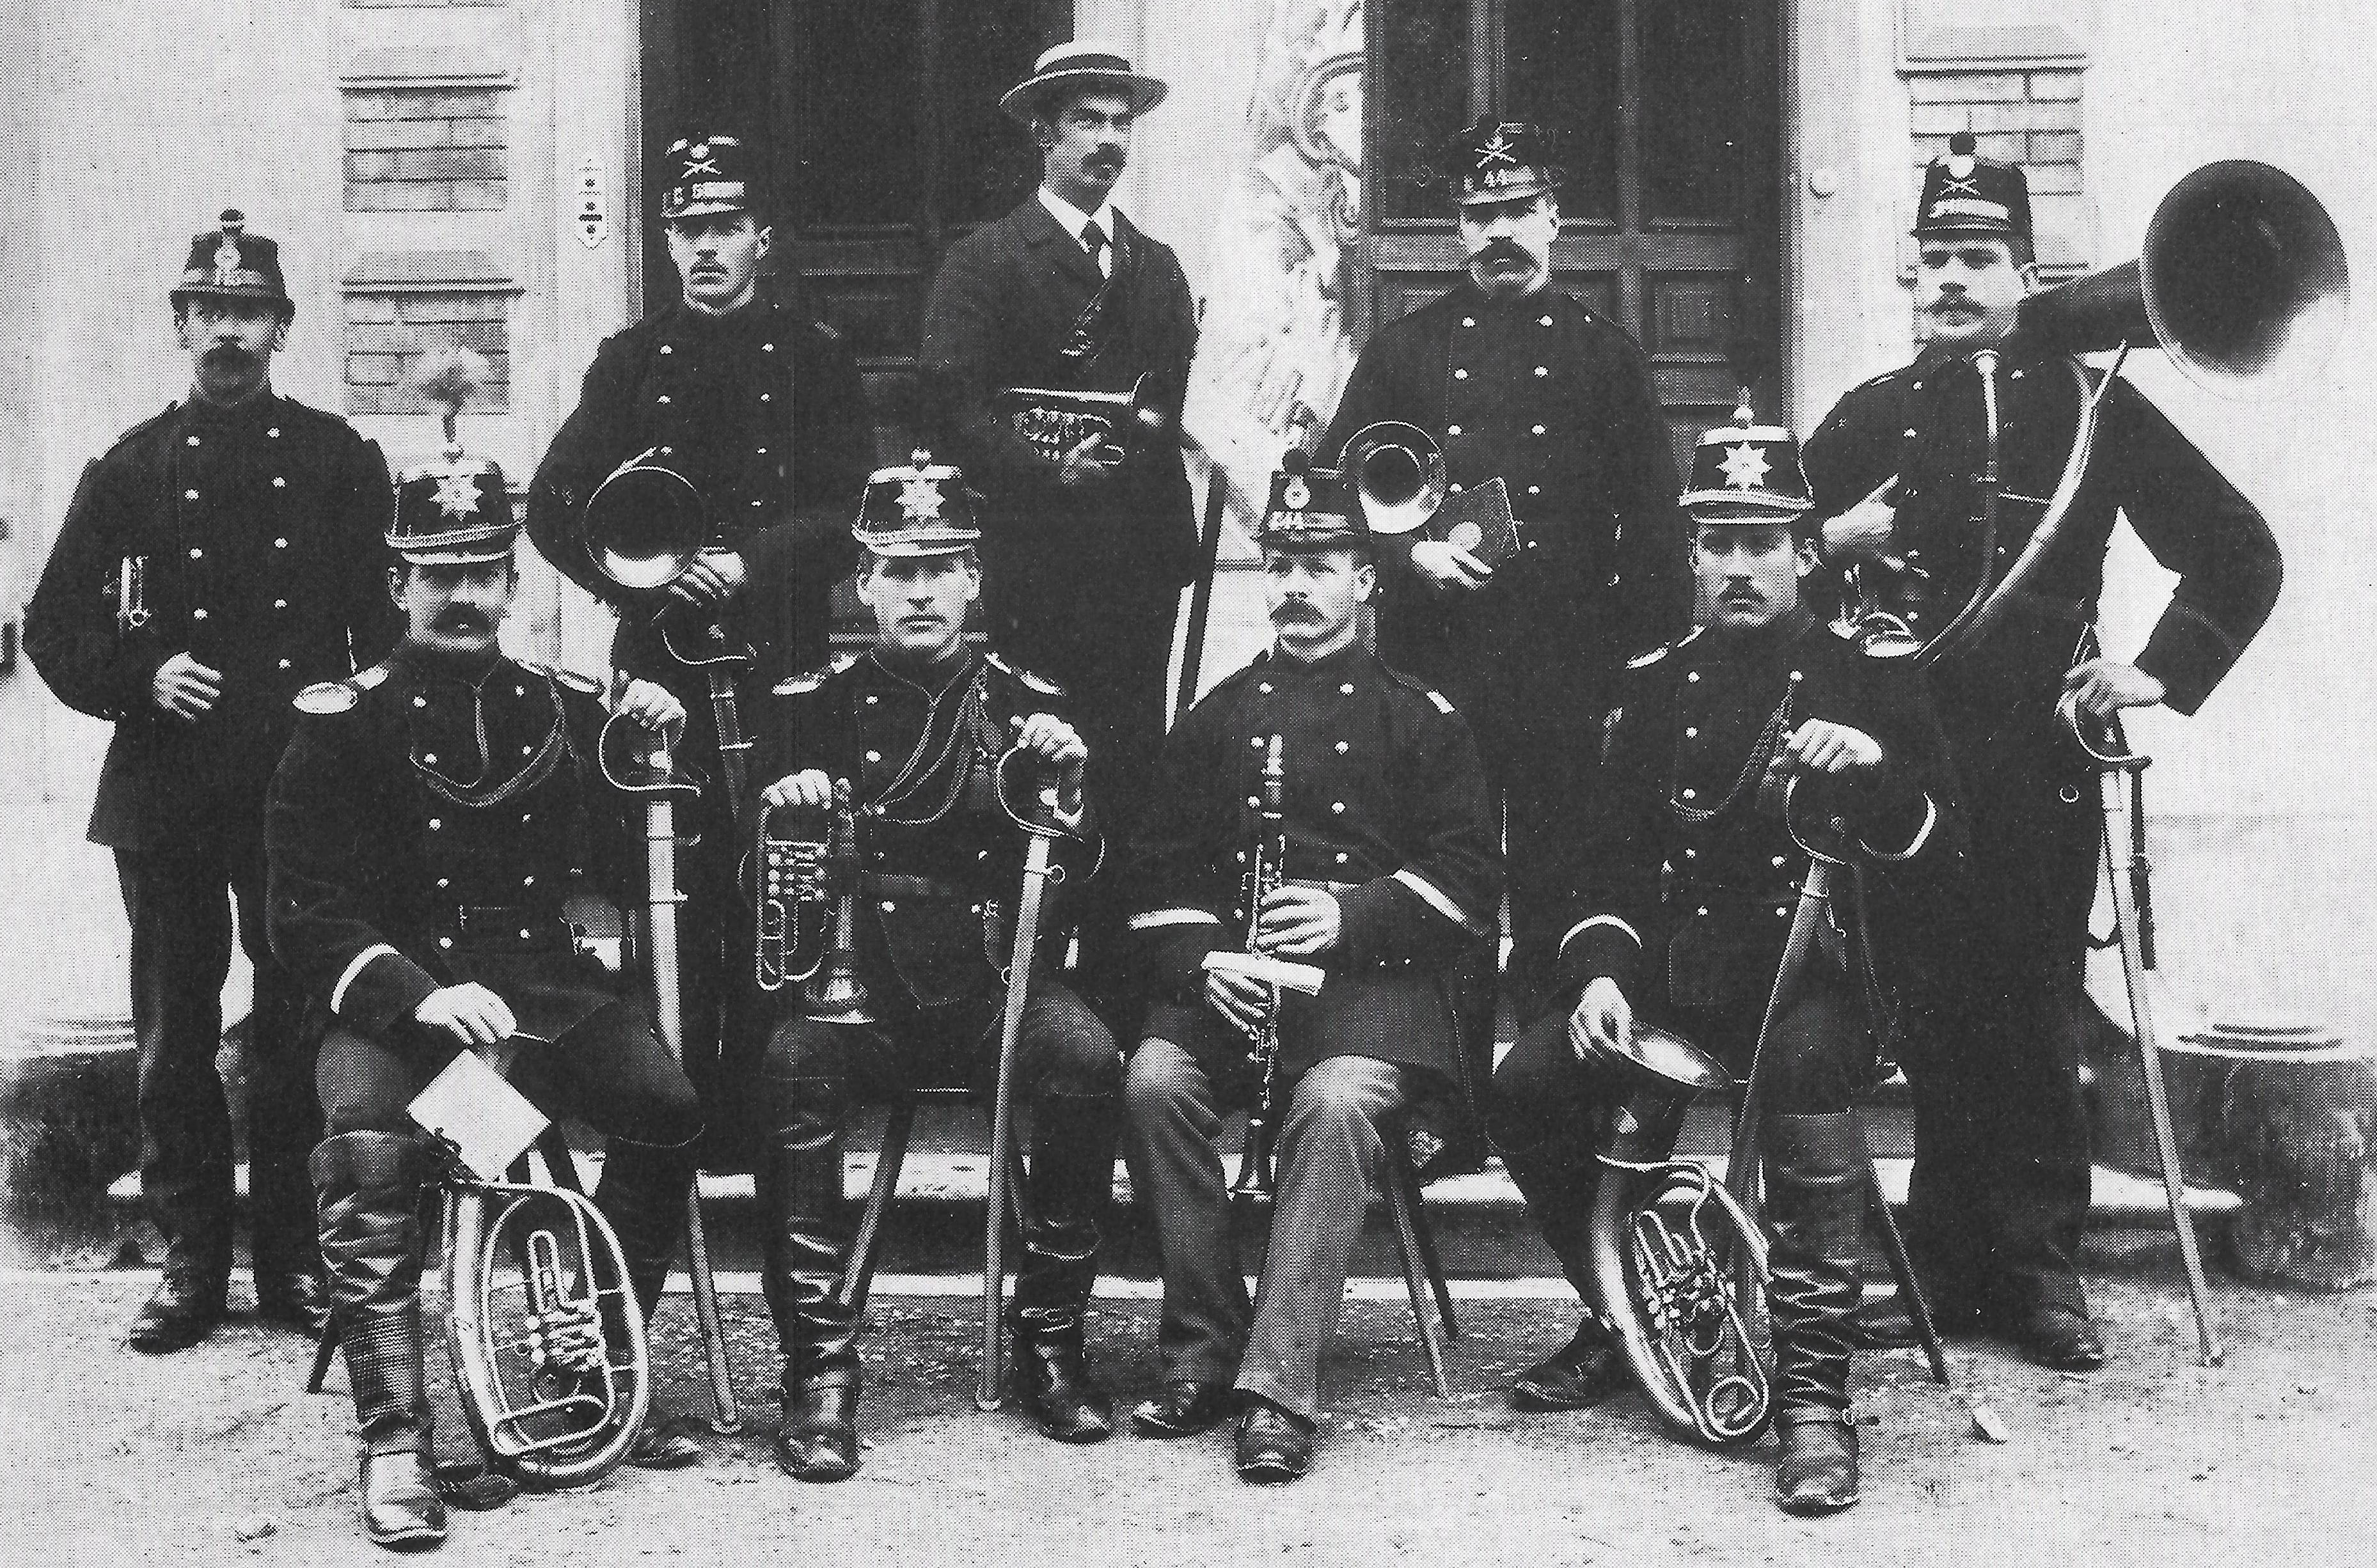
\includegraphics{./chap/1900-1925/MGH-1905.jpg}}
    \label{fig:mgh-1905}
    \caption{1905}
\end{figure}
\begin{figure}[h]
    \centerline{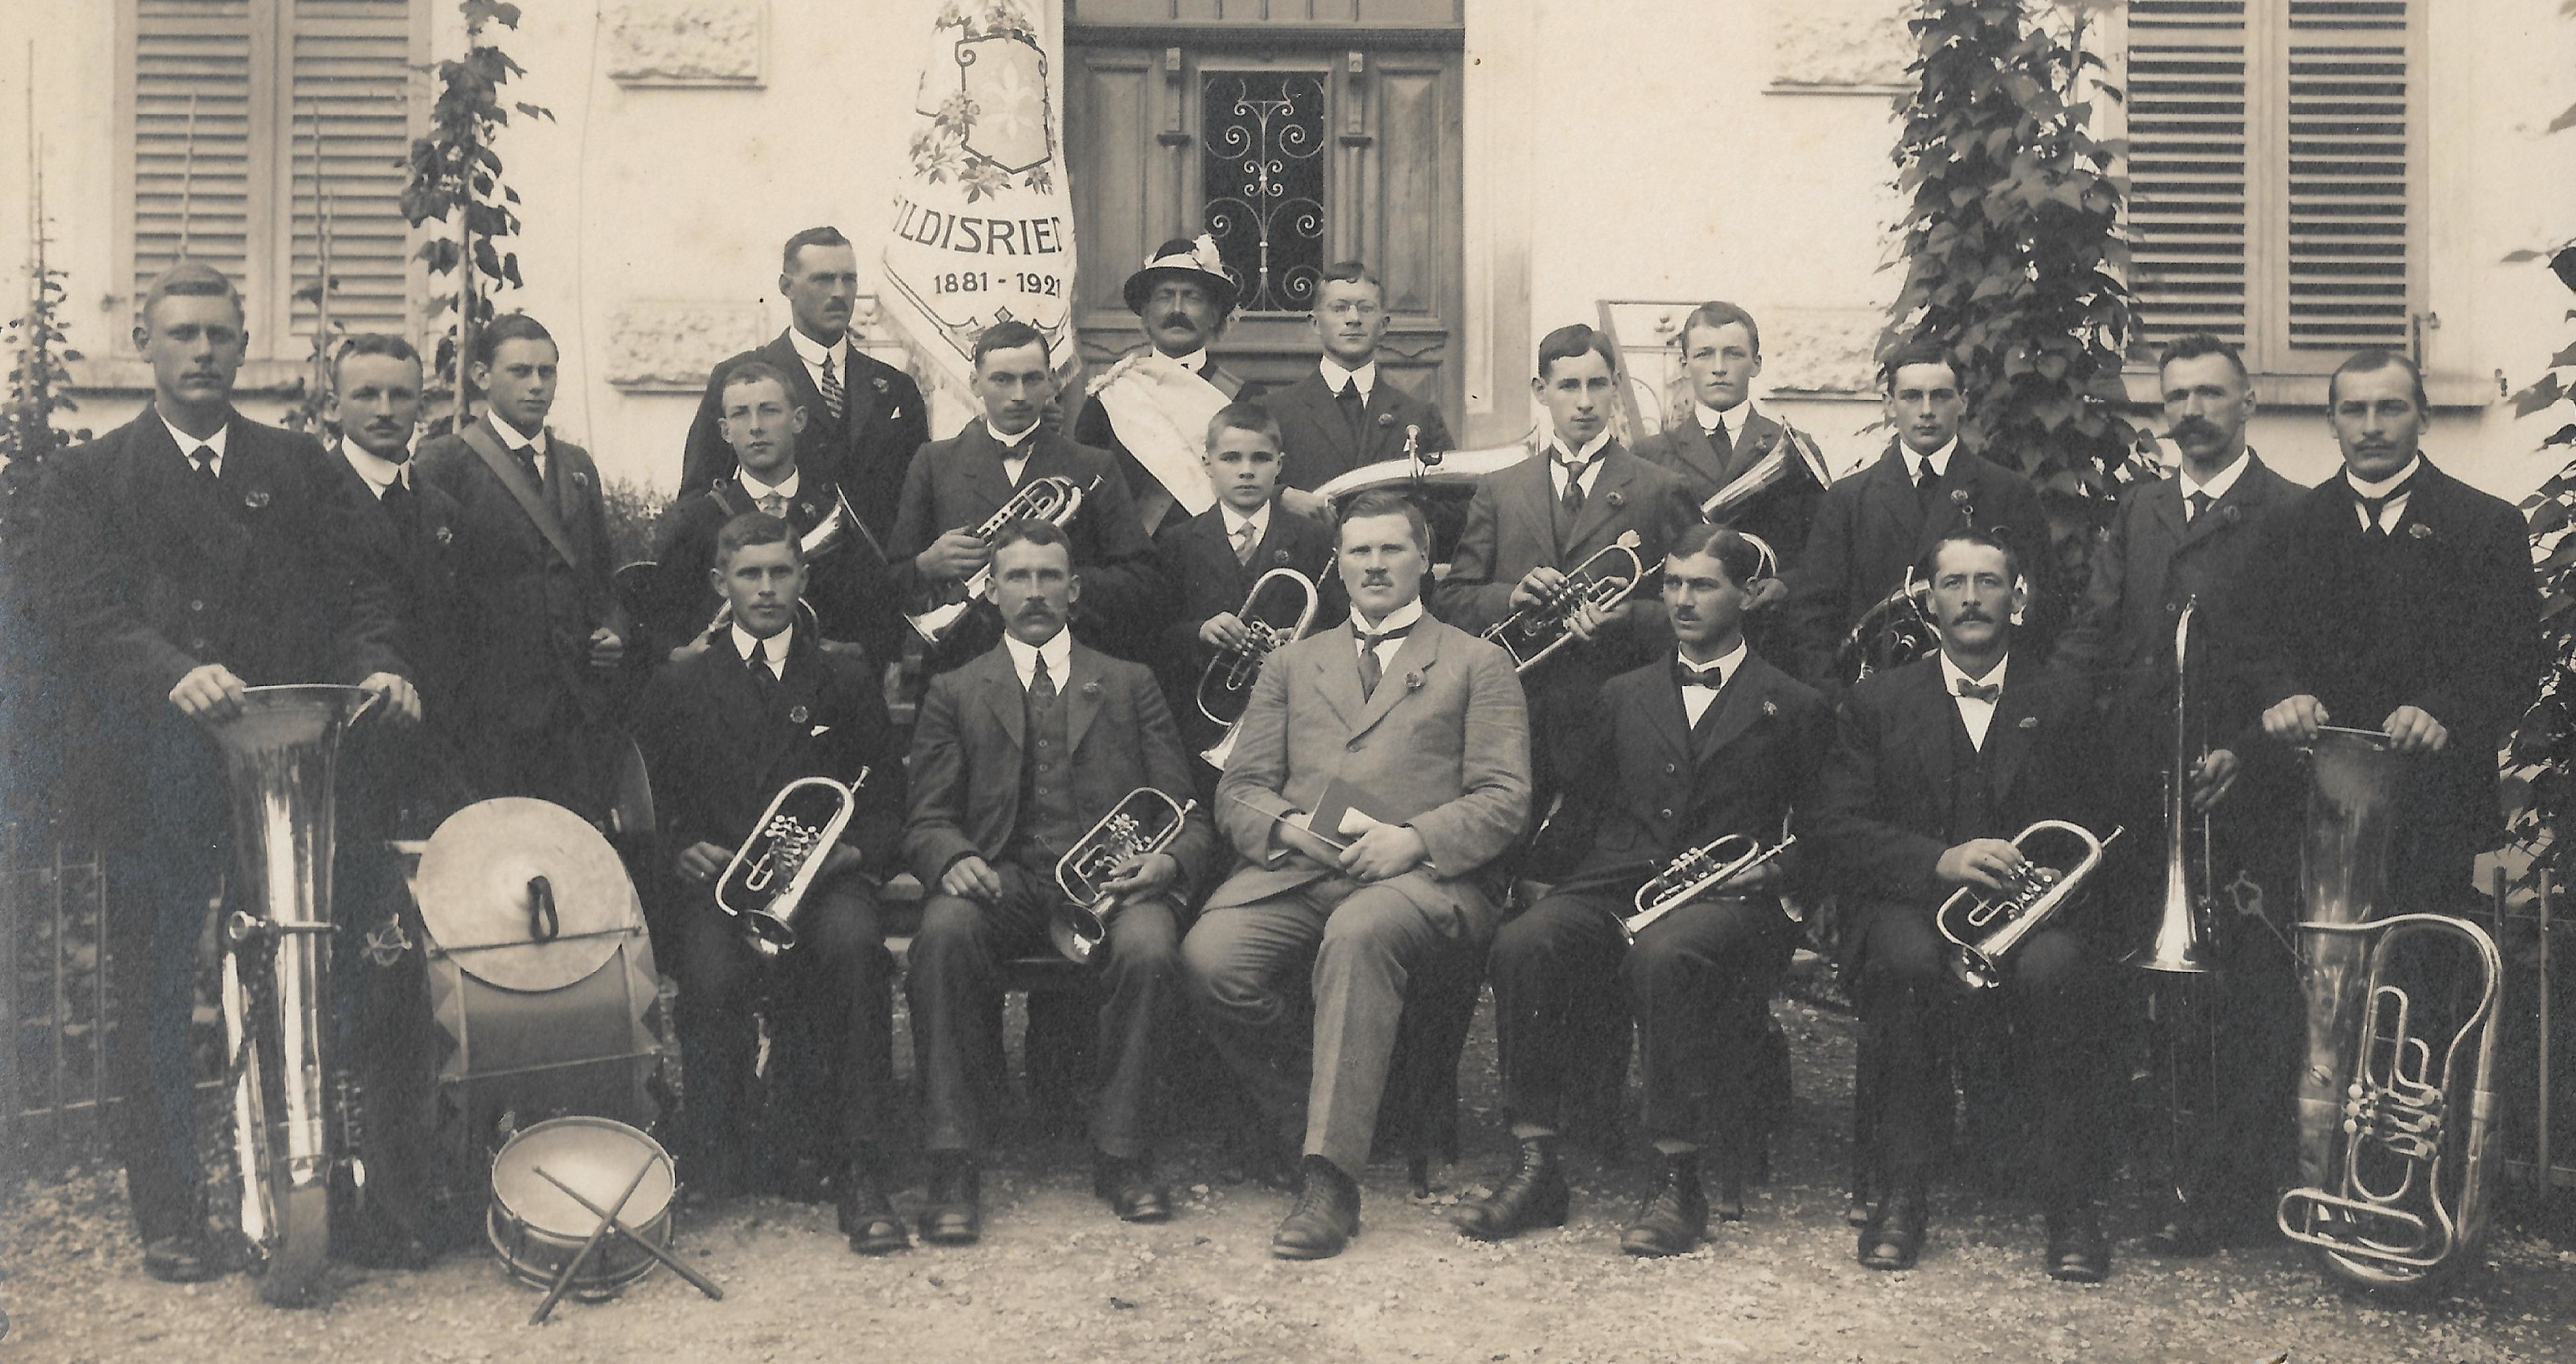
\includegraphics{./chap/1900-1925/MGH-1921.jpg}}
    \label{fig:mgh-1921}
    \caption{1921}
\end{figure}


\groupphoto{0.93}{0.8}{./chap/1900-1925/MGH-1905.jpg}
{\emph{Erstes Vereinsfoto 1905}\\
    Von links nach rechts sitzend:\\
    Estermann Josef, Halden, Troxler Xaver, Wiederkehr, Muff Peter, Lehrer,
    Troxler Kaspar, Moos\\
    Von links nach rechts stehend:\\
    Bühlmann Rudolf, Hermetsmatt, Müller Heinrich, Dorf, Estermann Heinrich,
    Traselingen, Suter Kaspar, Dorf, Suter Hans-Georg, Dorf} {fig:mgh-1905}

\begin{history}

    % \subsection*{1900-1925}

    Wenn auch diese Zeitspanne Mitgliederwechsel brachte, so konnte doch ein
    langsames Wachsen und Gedeihen der Musikgesellschaft festgestellt werden.
    Ihre Mitgliederzahl erhöhte sich von zehn auf neunzehn Mann. Die Tätigkeit
    bestand in den ersten Jahren noch vorwiegend aus dem Musizieren bei
    Ständchen, Ausmärschen und Tanzanlässen.

    Dass die Musikgesellschaft Hildisrieden bemüht war, gute Beziehungen zu
    Kirchenchor und Schützengesellschaft zu pflegen, beweisen die gemeinsamen
    Konzerte und Ausflüge auf die Rigi, nach Engelberg und Andermatt. Die Musik
    betrachtete ihre Aufgabe aber nicht bloss im Tanzmusikspielen, Sie war
    jederzeit bereit aufzutreten, wenn sich irgendetwas tat in der Gemeinde. Das
    zeigte die Einweihungsfeier unserer neuen Kirche im Jahre 1904. Der Verein
    war bestrebt, diesem Anlass ein festliches Gepräge zu geben und erfreute mit
    seinen Beiträgen den Bischof Leonard Haas und all die vielen Gäste.

    Im Verlaufe des Herbstes gleichen Jahres wurde die Gesellschaft zur
    Unterhaltung zu einem Grossanlass nach Münster aufgeboten. Es ging um das
    umstrittene Wynentalbahn-Projekt, das damals viel Gesprächsstoff lieferte,
    hätte doch die Weiterführung der Linie über Hildisrieden bis Emmenbrücke
    unser Dorf in der Entwicklung beeinflusst. (Geplanter Bahnhof bei der
    heutigen Bäckerei Arnold).

    Die Musikgesellschaft wurde 1905 erstmals photografiert.

    Dass der Probenbesuch nicht immer den Wünschen des Kapellmeisters entsprach,
    zeigt das Probenverzeichnis von 1907. Von den 15 abgehaltenen Proben trug
    nur eine den Vermerk \enquote{Alle anwesend}. Stets war die Musik bereit,
    ihren Möglichkeiten entsprechend mitzuwirken, so 1909 am Pfarraufritte von
    Pfarrer Alois Hodel.

    In den Jahren 1910 und 1911 sind nebst den kirchlichen und den weltlichen
    Anlässen keine weiteren Taten zu verzeichnen, ebenso schweigt das
    Probenverzeichnis.

    An der Generalversammlung vom 31. März 1912 wurden die Statuten wieder
    revidiert und von folgenden Mitgliedern unterzeichnet:

    \noindent
    Karl Estermann, Traselingen\\
    Peter Muff, Lehrer\\
    Alois Estermann, Traselingen\\
    Kaspar Troxler, Moos\\
    Kaspar Suter, Dorf\\
    Alois Troxler, Schopfen\\
    Franz Troxler, Schopfen\\
    Josef Troxler, Schopfen\\
    Alois Wolf, Sandgütsch\\
    Josef Gassmann, Gigen\\
    Balz Gassmann, Gigen\\
    Heinrich Estermann, Dorf

    Der Rechnungsbericht, abgelegt von Kassier Kaspar Troxler, verzeigte an
    Einnahmen Fr. 298.90 und an Ausgaben Fr. 79.22. Die Mehreinnahmen wurden
    verteilt, und jedes Mitglied konnte 15 Franken als \enquote{Dividende}
    entgegennehmen.

    Dass die Musikgesellschaft 1915 neue Mitglieder aufnehmen konnte, bezeugt,
    dass der Verein bestrebt war, sich weiterzuentwickeln und an sich zu
    arbeiten. Neu wurden in den Verein aufgenommen: Josef Disler, Dorf; Jakob
    Estermann, Bethlehem; Heinrich Estermann, Ohmenlingen; Heinrich Estermann,
    Dorf; Josef Jutz, Löwen, und Leo Erni, Schmiede.

    Diese Mitglieder haben das Vereinsschifflein in gesellschaftlicher Hinsicht
    wieder belebt und flotte Probenarbeit geleistet. Die Musikgesellschaft hatte
    sich nun schon derart gefestigt, dass der entfachte Weltkrieg das
    Vereinsleben nicht mehr zum Stillstand zu bringen vermochte. Bei jeder, wenn
    auch nur selten sich bietenden Gelegenheit, wurden Proben abgehalten.

    Im Jahre 1915 hatte der Vorstand folgendes Aussehen:

    \noindent
    Präsident: Kaspar Suter, Dorf\\
    Dirigent Alois Estermann, Traselingen\\
    Aktuar: Karl Estermann, Traselingen\\
    Kassier: Kaspar Troxler, Moos\\
    Mitglied: Alois Troxler, Lenzenhof

    \enquote{Friede ist es zwar geworden, das Elend und der Hass unter den
        Völkern ist geblieben}, so beginnt der Tätigkeitsbericht von 1919,
    Arbeitslosigkeit und Unzufriedenheit herrschten in der Heimat. Als in
    den ersten Augusttagen das tapfere Inf Reg 19 nach Zürich gerufen wurde,
    um Ruhe und Ordnung zu schaffen, betraf das auch Hildisrieder
    Musikanten,

    Am Jubiläumsschiessen der Schützengesellschaft Hildisrieden gab die Musik im
    Löwen ein Konzert zum besten.

    Das Symbol des Vereins, die Fahne, die 40 Jahre Wind und Wetter getrotzt
    hatte, sollte ersetzt werden. Eine von Frauen und Töchtern Hildisriedens im
    Frühjahr 1921 durchgeführte Sammlung, ermöglichte dieses Vorhaben. Besondere
    Aufmerksamkeit schenkte man der Musikgesellschaft bei der Teilnahme am
    Kantonalen Musiktag in Sempach unter der Leitung von Lehrer Alois Troxler.

    An der Gemeindeversammlung vom 25. März 1924 beantragte Josef Disler sen.,
    dass der jährliche Beitrag der Gemeinde von Fr. 40.— auf Fr. 100,— erhöht
    werden sollte, was auch einstimmig genehmigt wurde. Von nun an wurde
    intensiver und freudiger musiziert.

    \subsubsection*{Zweite Fahnenweihe 1921}

    Nachdem im Verlaufe der Generalversammlung vom 29. Mai 1921 der Wunsch nach
    einer neuen Fahne laut wurde, erhielt der Präsident Kaspar Suter den
    Auftrag, diese Angelegenheit nun ernsthaft an die Hand zu nehmen. Man war
    sich einig, dass die 40-jährige Fahne, die Wind und Wetter getrotzt hat,
    ersetzt werden sollte. Die nötige Geldsammlung wurde von acht Töchtern
    besorgt. Frl. Rosa Estermann, Grossrats, Ohmenlingen, stand als Präsidentin
    an der Spitze. Der abgelieferte Betrag von Fr. 1024.— übertraf alle
    Erwartungen und wurde dankbar entgegengenommen.\\
    \\
    Fahnenweihe vom 4. September 1921\\
    Mittags 14 Uhr Festzug vom Schulhaus zur Kirche; Josef Estermann, Halden,
    marschierte als Fähnrich mit verhüllter Fahne, umgeben von Ehrendamen,
    Patenpaars und Gästen in die Kirche. Im Chor wurde das Banner entrollt und
    vom Ortspfarrer Alois Hodel eingesegnet. Des schlechten Wetters wegen fand
    die Übergabe im Löwensaal statt. Voller Freude überreichten Heinrich
    Estermann, Ohmenlingen, als Götti und Elisabeth Zwinggi, von Schopfen, als
    Gotte ihren Musikfreunden das recht hübsch präsentierende Banner.

    Es trägt die Inschrift :\enquote{In Freud und Leid zum Spiel bereit}.

\end{history}


\begin{figure}[ht]
    \subfloat[Dorfplatz mit Vierwaldstätterhof]{%
        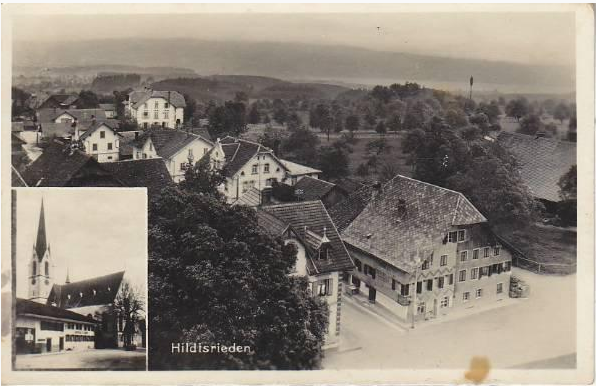
\includegraphics[height=0.5\textheight,keepaspectratio]{./Dorf-Bilder/p18}
    }\hfil
    \subfloat[Um 1920]{%
        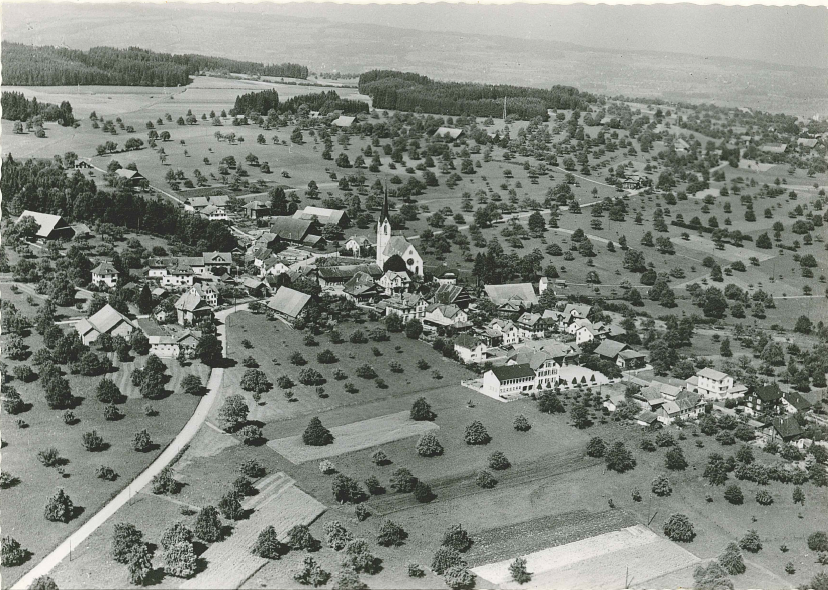
\includegraphics[height=0.5\textheight,keepaspectratio]{./Dorf-Bilder/p12}
    }
\end{figure}

\clearpage

\groupphoto{0.93}{0.8}{./chap/1900-1925/MGH-1921.jpg}
{ \emph{Die Musikgesellschaft 1921}\\
    Von links nach rechts sitzend:\\
    Estermann Heinrich, Troxler Kaspar, Troxler Alois, Dirigent, Estermann Alois,
    Troxler Alois\\
    1. Reihe stehend:\\
    Disler Josef, Estermann Heinrich, Suppiger Hans, Estermann Jakob, Zwinggi
    Josef, Suter Josef, Erni Leo, Zwinggi Jakob, Suter Kaspar, Gassmann Balz\\
    2. Reihe stehend:\\
    Estermann Karl, Estermann Josef, Estermann Jakob, Estermann
    Jakob}{fig:mgh-1921}

\begin{figure}[!ht]
    \centerline{
        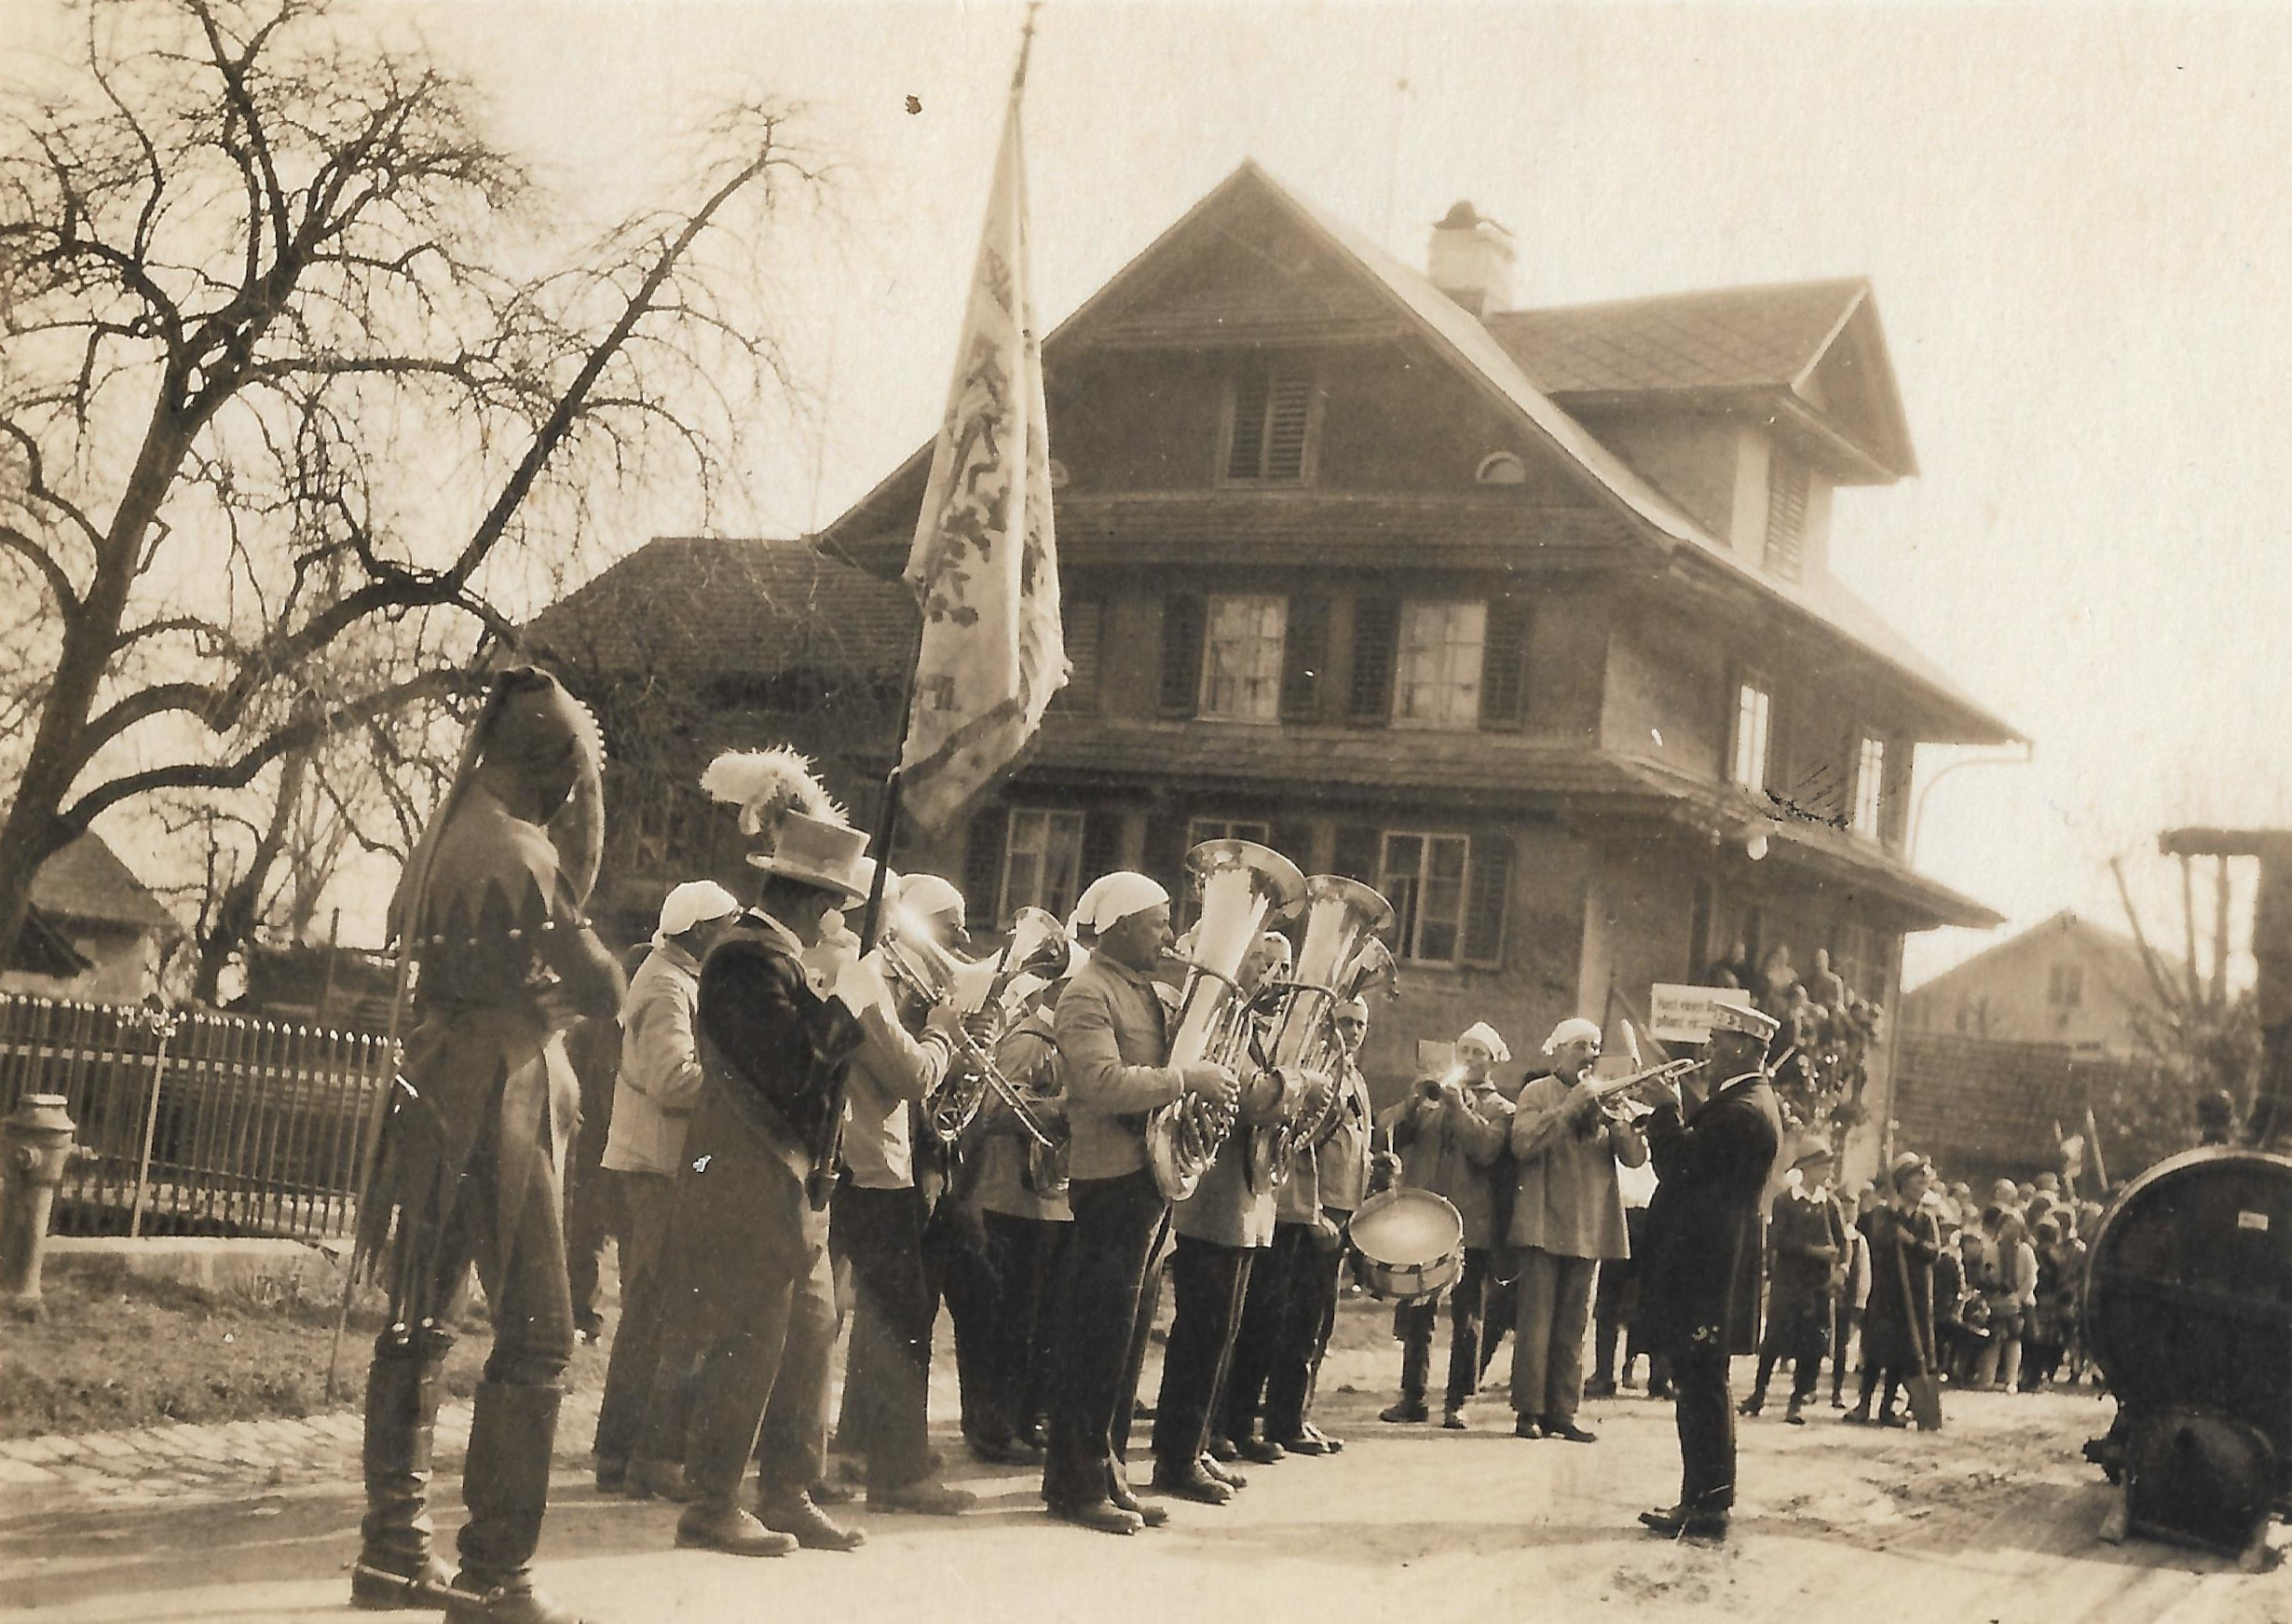
\includegraphics{./chap/1900-1925/Fasnacht-1920er-1.jpg}
        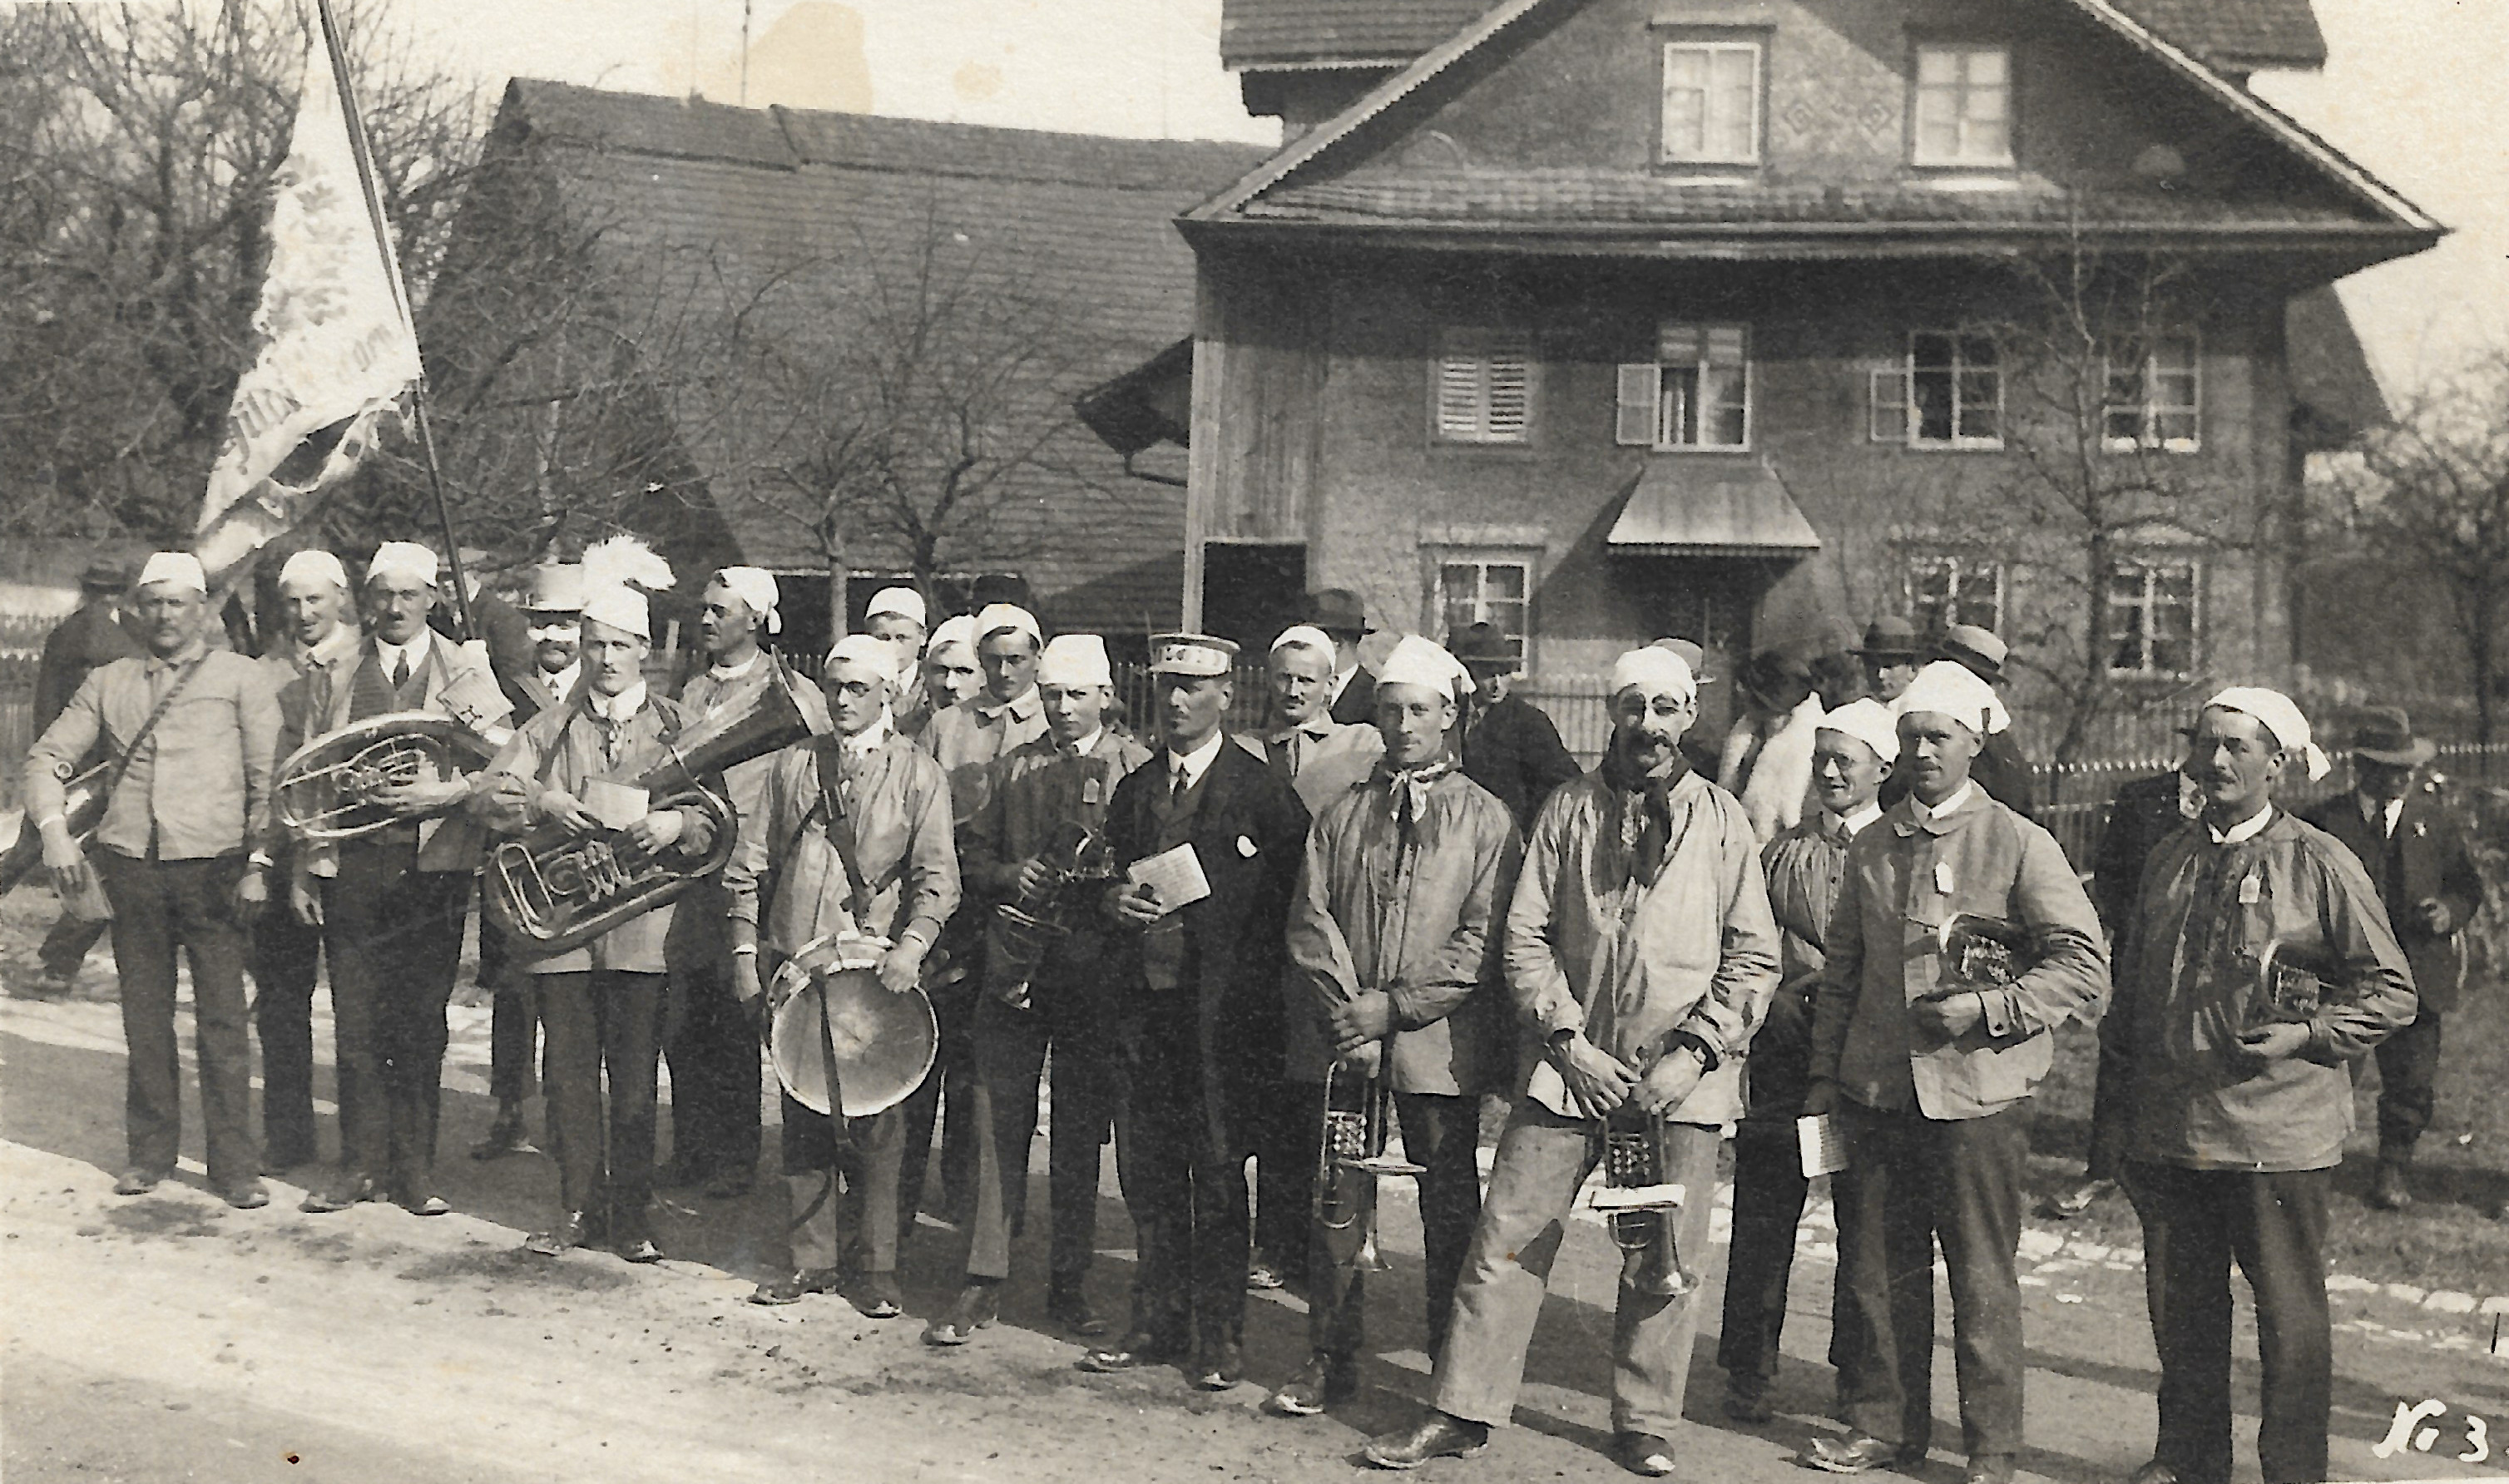
\includegraphics{./chap/1900-1925/Fasnacht-1920er-2.jpg}}
    \label{fig:mgh-fasnacht-1920}
    \caption{Fasnacht in den 1920ern}
\end{figure}


\begin{figure}[h]
    \centerline{
        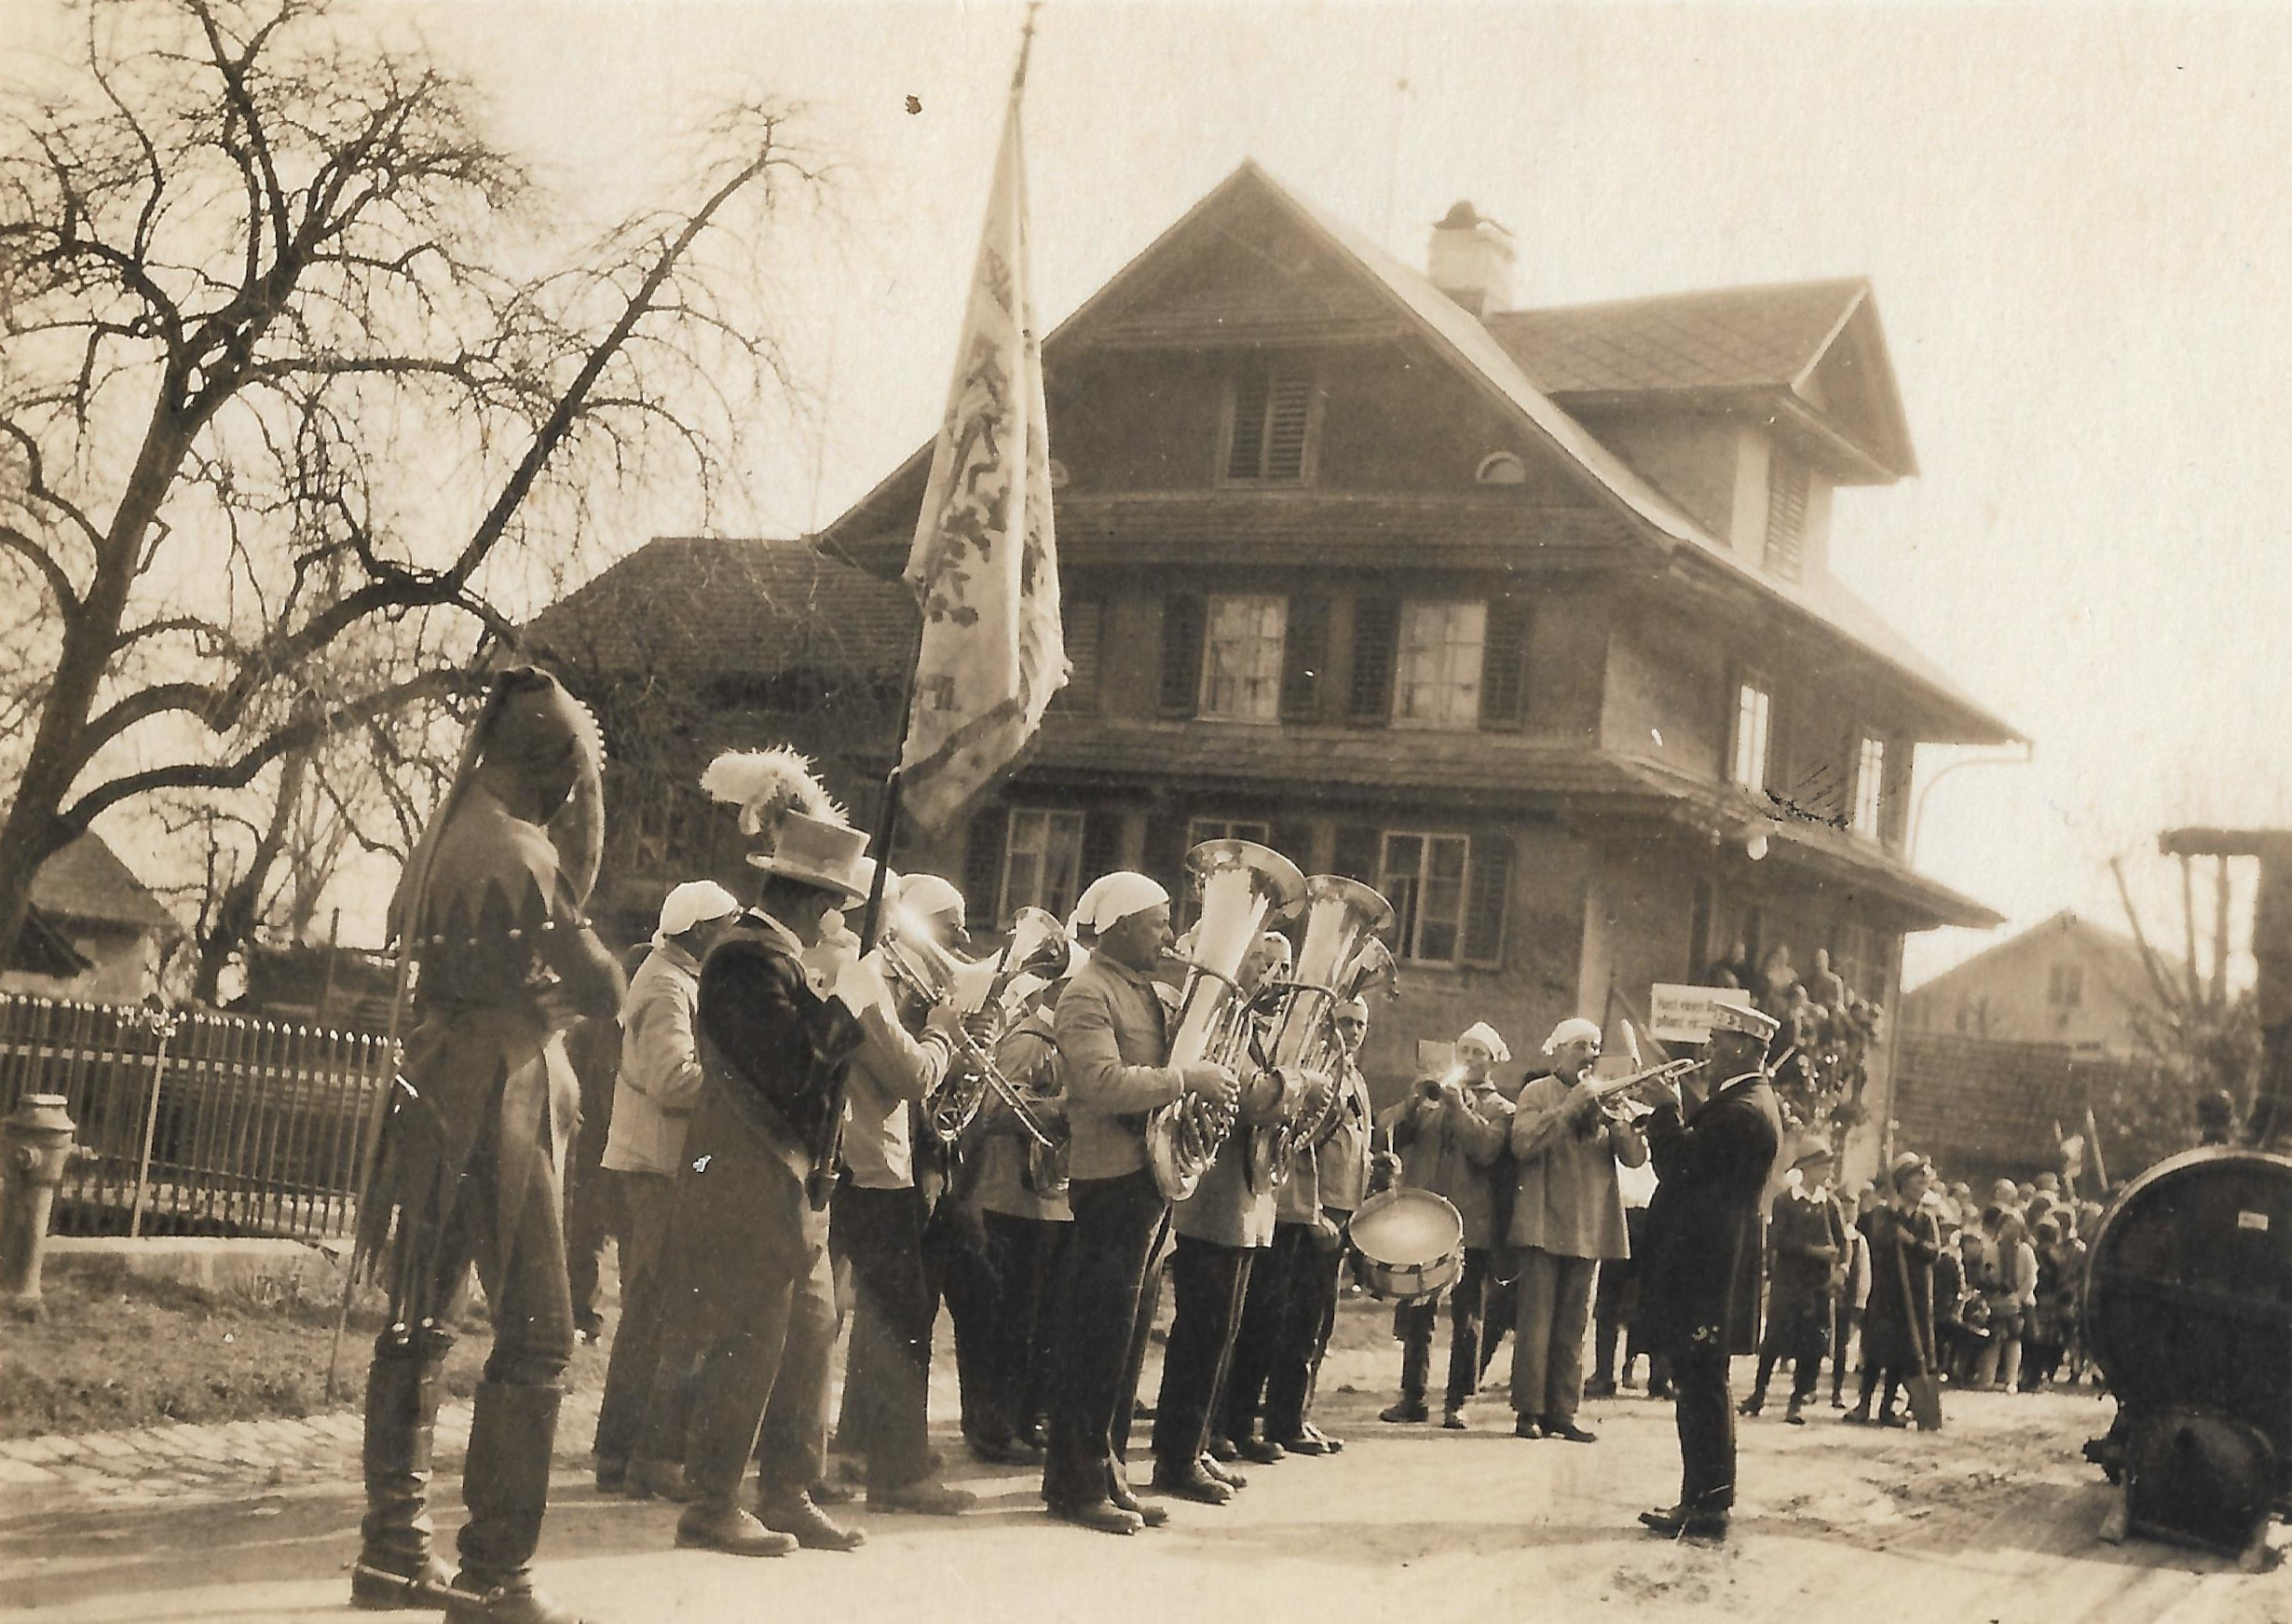
\includegraphics{./chap/1900-1925/Fasnacht-1920er-1.jpg}
        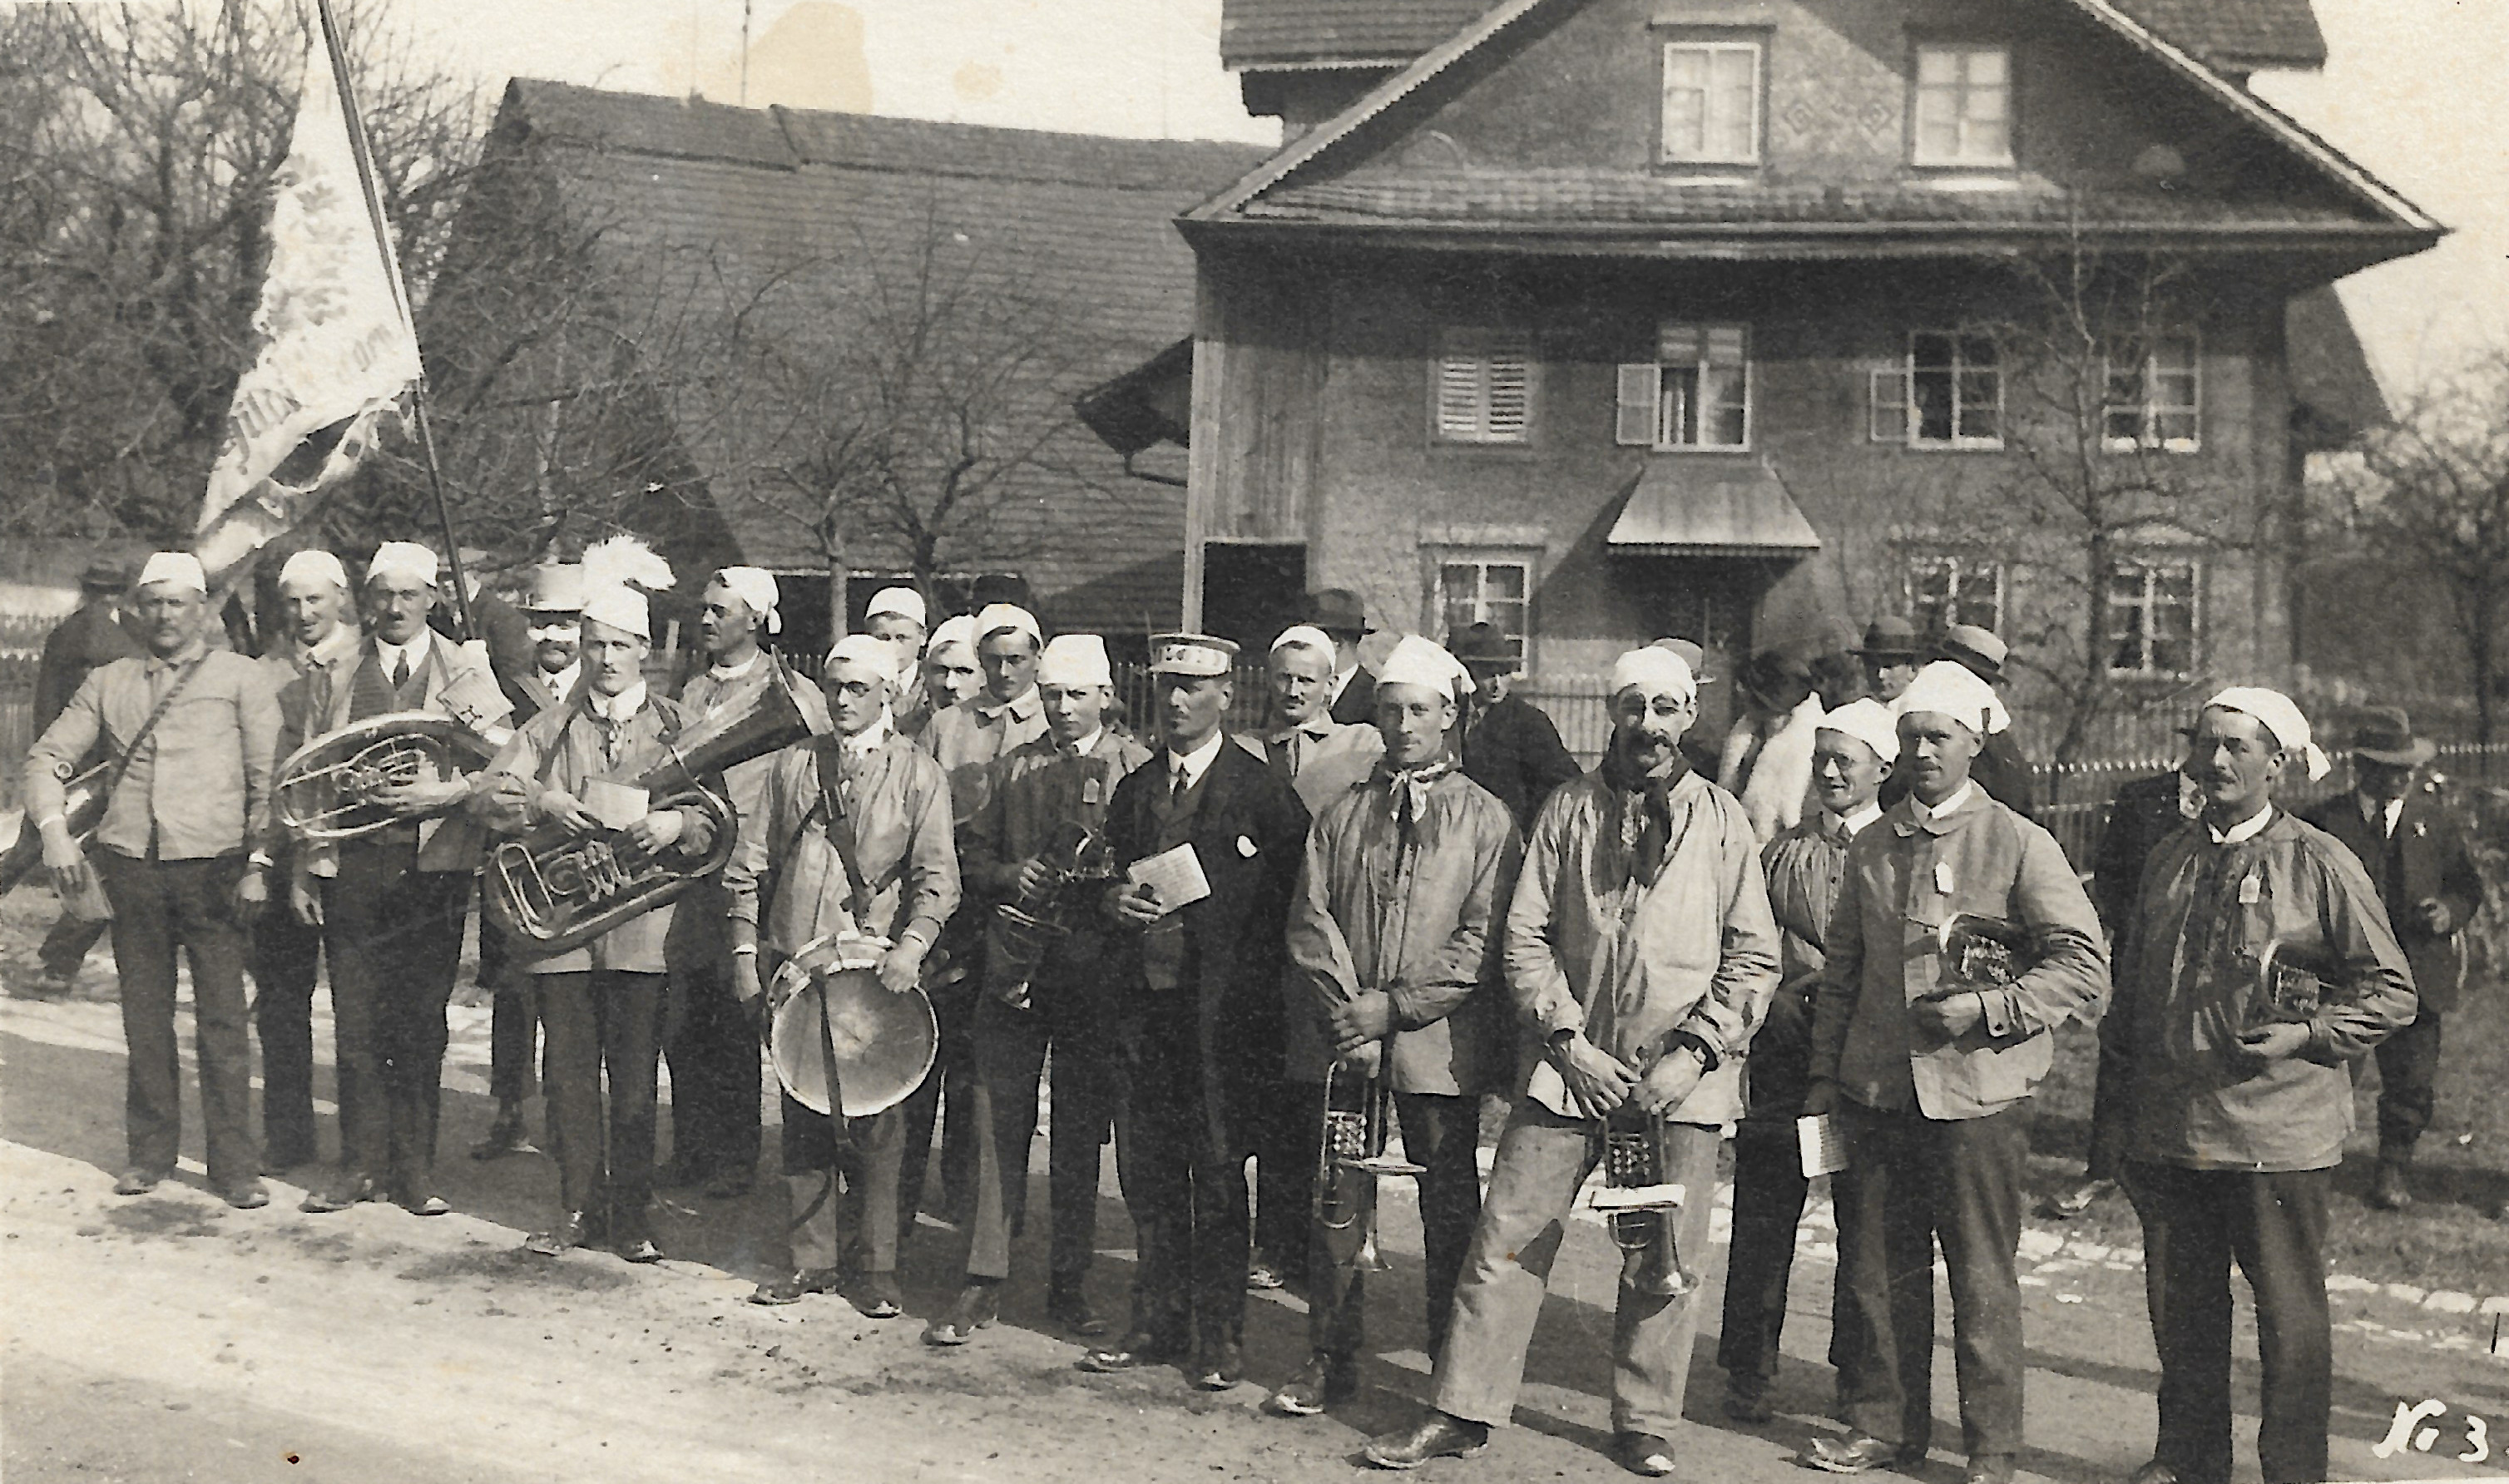
\includegraphics{./chap/1900-1925/Fasnacht-1920er-2.jpg}}
    \label{fig:mgh-fasnacht-1920}
    \caption{Fasnacht in den 1920ern}
\end{figure}
\clearpage

\section{1925-1950}
\begin{figure}[p]
    \centering
    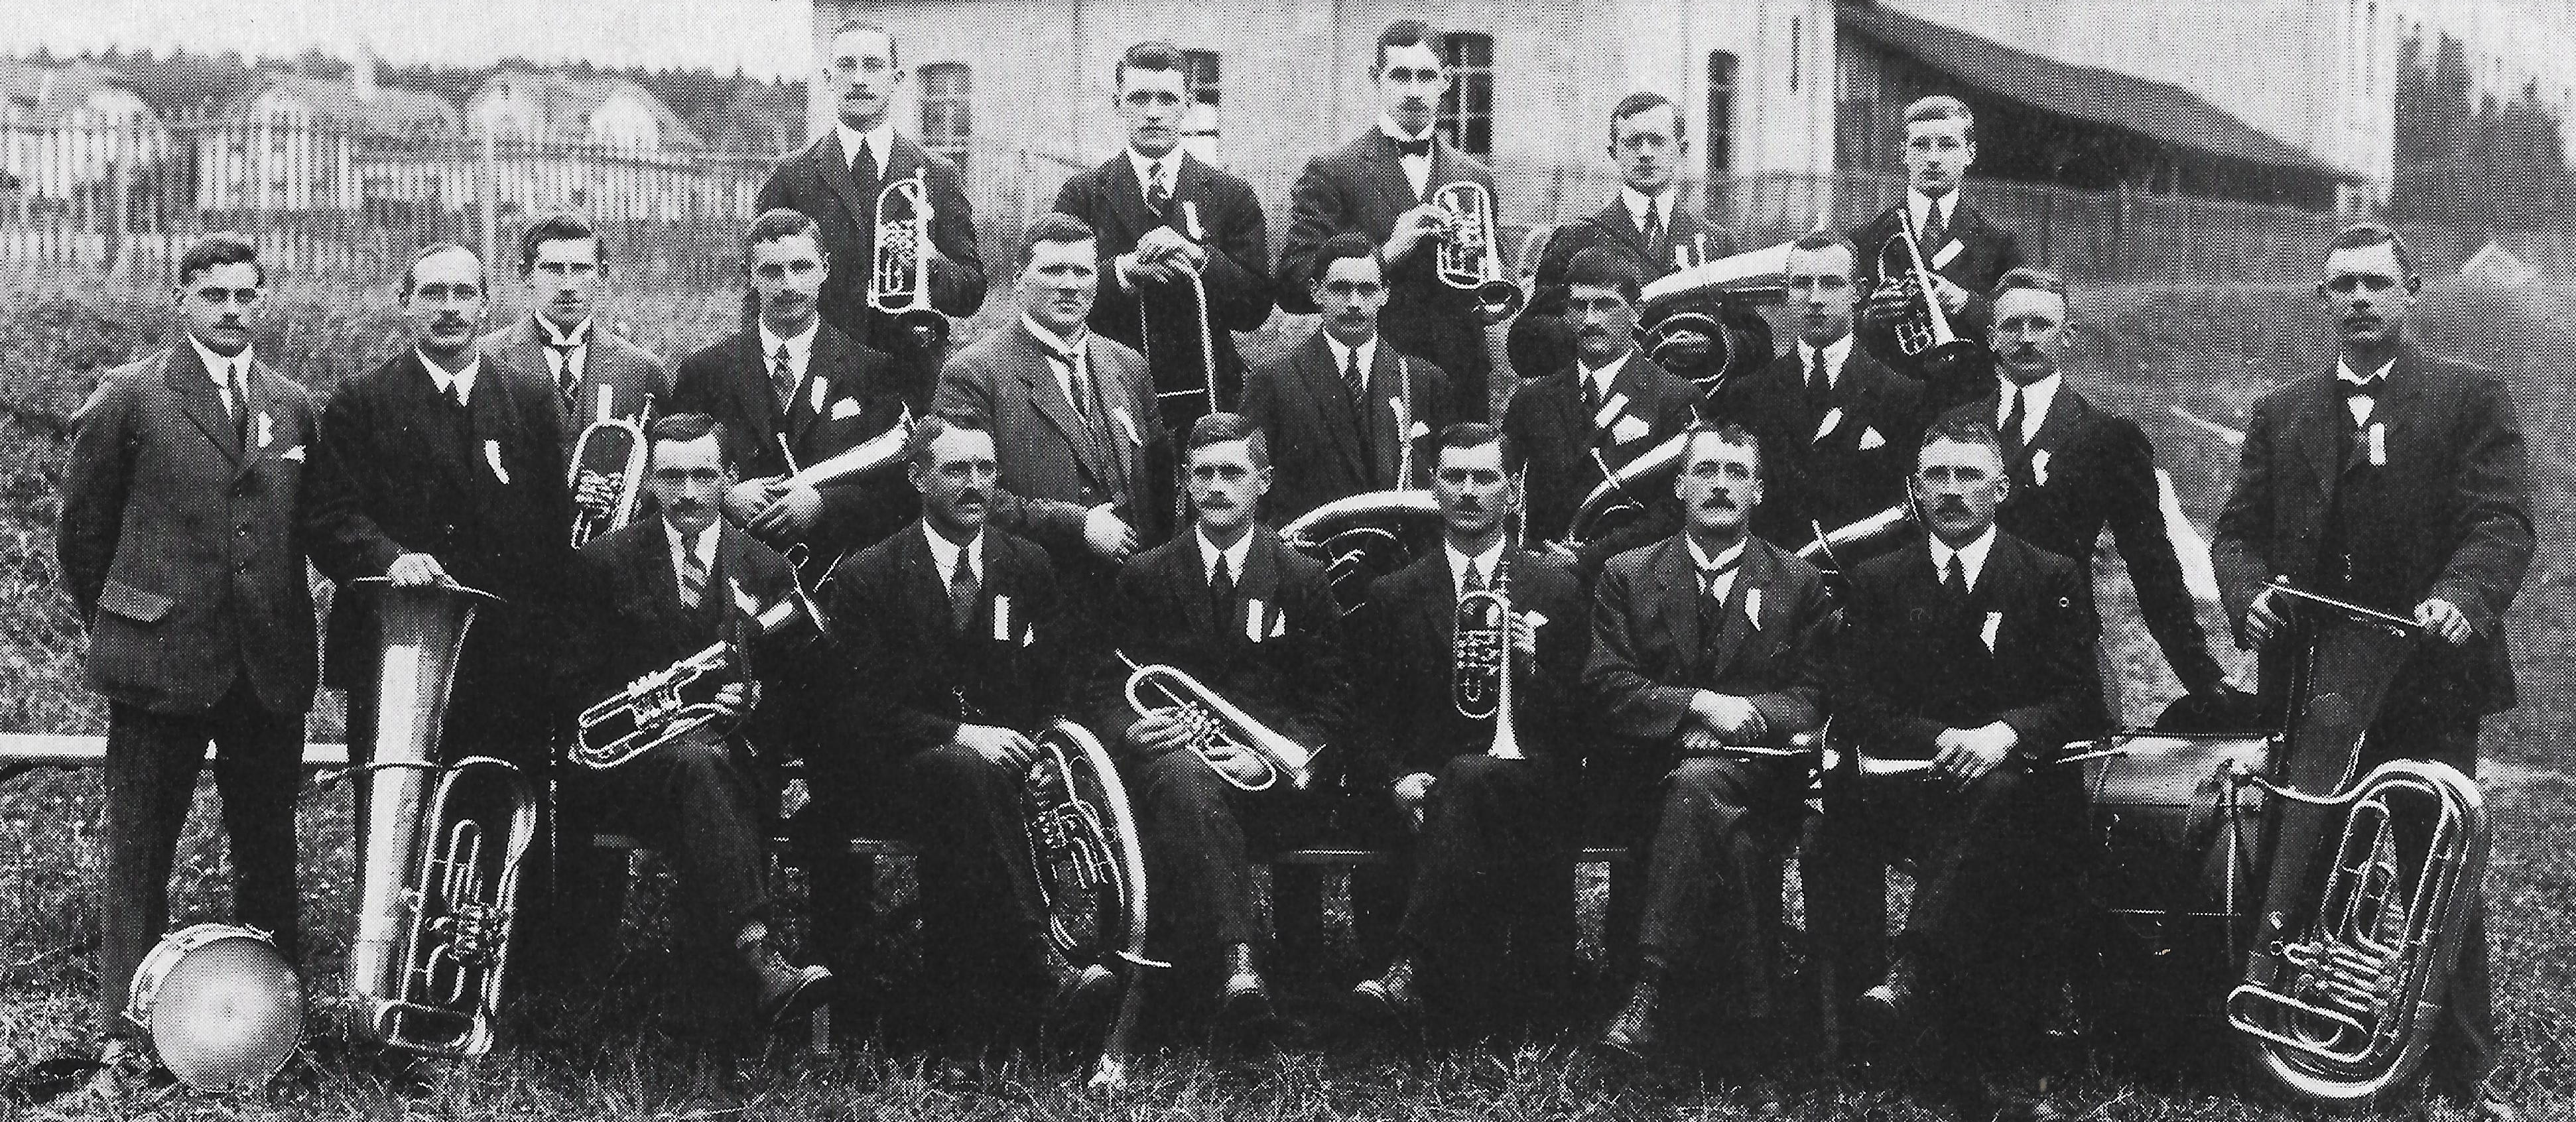
\includegraphics{./chap/1925-1950/MGH-1926.jpg}
    \label{fig:mgh-1926}
    \caption{1926}
\end{figure}
\begin{history}

    % \subsection{1925-1950}

    In diesem Vierteljahrhundert machte die Musikgesellschaft auf musikalischem
    Gebiet grosse Fortschritte. In diese Zeitspanne fallen die Besuche der
    Musikanlässe ‘von Hochdorf, Rickenbach, Wolhusen, Willisau, 'Ebikon, Rain
    und an das Eidg. Musikfest in St. Gallen. Die Teilnahme an diesen Festen,
    welche an die Direktion und an die Bläser hohe Anforderungen stellte, liess
    erkennen, dass der Verein gewillt war, eine höhere Stufe zu erreichen und
    nach Möglichkeit diese zu halten. Die vermehrte und auf Blasmusik
    zugeschnittene Literatur verlangte intensivere Probenarbeit. Tüchtiges und
    zielbewusstes Schaffen brachte der Musikgesellschaft Hildisrieden Lorbeeren
    ein, auf die sie sicher stolz sein konnte,

    Ausser dem Besuch von Musikfesten fand der Verein noch Zeit, an
    verschiedenen Veranstaltungen mitzuwirken. So treffen wir ihn 1929 am
    Festzug des Schweiz. Katholikentages in Luzern, als Festmusik an der
    Pferde-Springkonkurrenz und 1943 an der Vereranentagung des
    Kantonal-Schützenverbandes in Hildisrieden.

    An der Generalversammlung von 1932 wurde der Vorstand für eine weitere
    Amtsdauer (von 2 Jahren) bestätigt:

    Präsident: Josef Disler, Dorf Vize-Präsident: Alois Estermann, Traselingen
    Aktuar: Karl Estermann, Traselingen Kassier: Heinrich Estermann, Oele
    Beisitzer: Leo Erni, Wirt zum Kreuz. Jakob Estermann, Dorf Dirigent: Alois
    Estermann, Traselingen


    Eine besondere Anerkennung sei hier kurz der Vereinsführung gezollt. Im
    Vorstand treffen wir bis 1945 keinen Wechsel von grosser Bedeutung. Man fand
    stets wieder die geeignete Person, um entstandene Lücken zu füllen. Josef
    Disler, welcher der Musikgesellschaft volle 17 Jahre vorstand, wurde zum
    Dank für die geleisteten treuen Dienste zum Ehrenpräsidenten ernannt.

    Dass in einer Uniform der Musikant erst so recht zur Geltung kommt, ist
    altbekannt. Die Finanzierung der Neu-Uniformierung konnte die Kasse nicht
    verkraften. Durch eine Sammelaktion wurde der benötigte Betrag aufgebracht.

    Das Jahr 1939 brachte der Musikgesellschaft etwas Ungewolltes. Die in diesem
    Jahre ausgebrochene Maul- und Klauenseuche verhinderte einen geordneten.
    Probenbetrieb. Aber der im September entfachte Zweite Weltkrieg, der die
    Grosszahl der Mitglieder an die Grenze rief, wirkte nicht weniger hemmend.
    Die Musikgesellschaft hatte die Ehre, damals schon eine stattliche Zahl
    Militärtrompeter zu stellen, die während der langen Aktivdienstzeit
    musikalische Weiterbildung genossen.

    Solange die Musikgesellschaft bestand, fehlte sie nie an einer kirchlichen
    Feier. Am Fronleichnamstag 1940 aber waren so viele Musikanten an der
    Grenze, dass der Verein ausserstande war, die Prozession würdig zu
    gestalten. Das Spiel des Inf Reg 86, das in Hildisrieden einquartiert war,
    gab dem Allerheiligsten das Geleit und bekundete so die Verbundenheit von
    Volk und Armee.

    Im Frühjahr 1945 nahm der mörderische Krieg, der so viele Tränen fliessen
    liess, endlich ein Ende. Der denkwürdige 8. Mai wurde zum
    Waffenstillstandstag erklärt. Mit dem Wegfall des Aktivdienstes begann
    wieder ein regelmässiges Vereinsleben mit Probenbetrieb in alter Form. Der
    neu gewählte Präsident, Josef Rüttimann, wurde allen Aktiven ein Vorbild.

    1949 war für die Musikgesellschaft ein Jubeljahr. Der fünfundsiebzigste
    Geburtstag wurde gebührend gefeiert.


\end{history}

\begin{figure}[h]
    \centerline{
        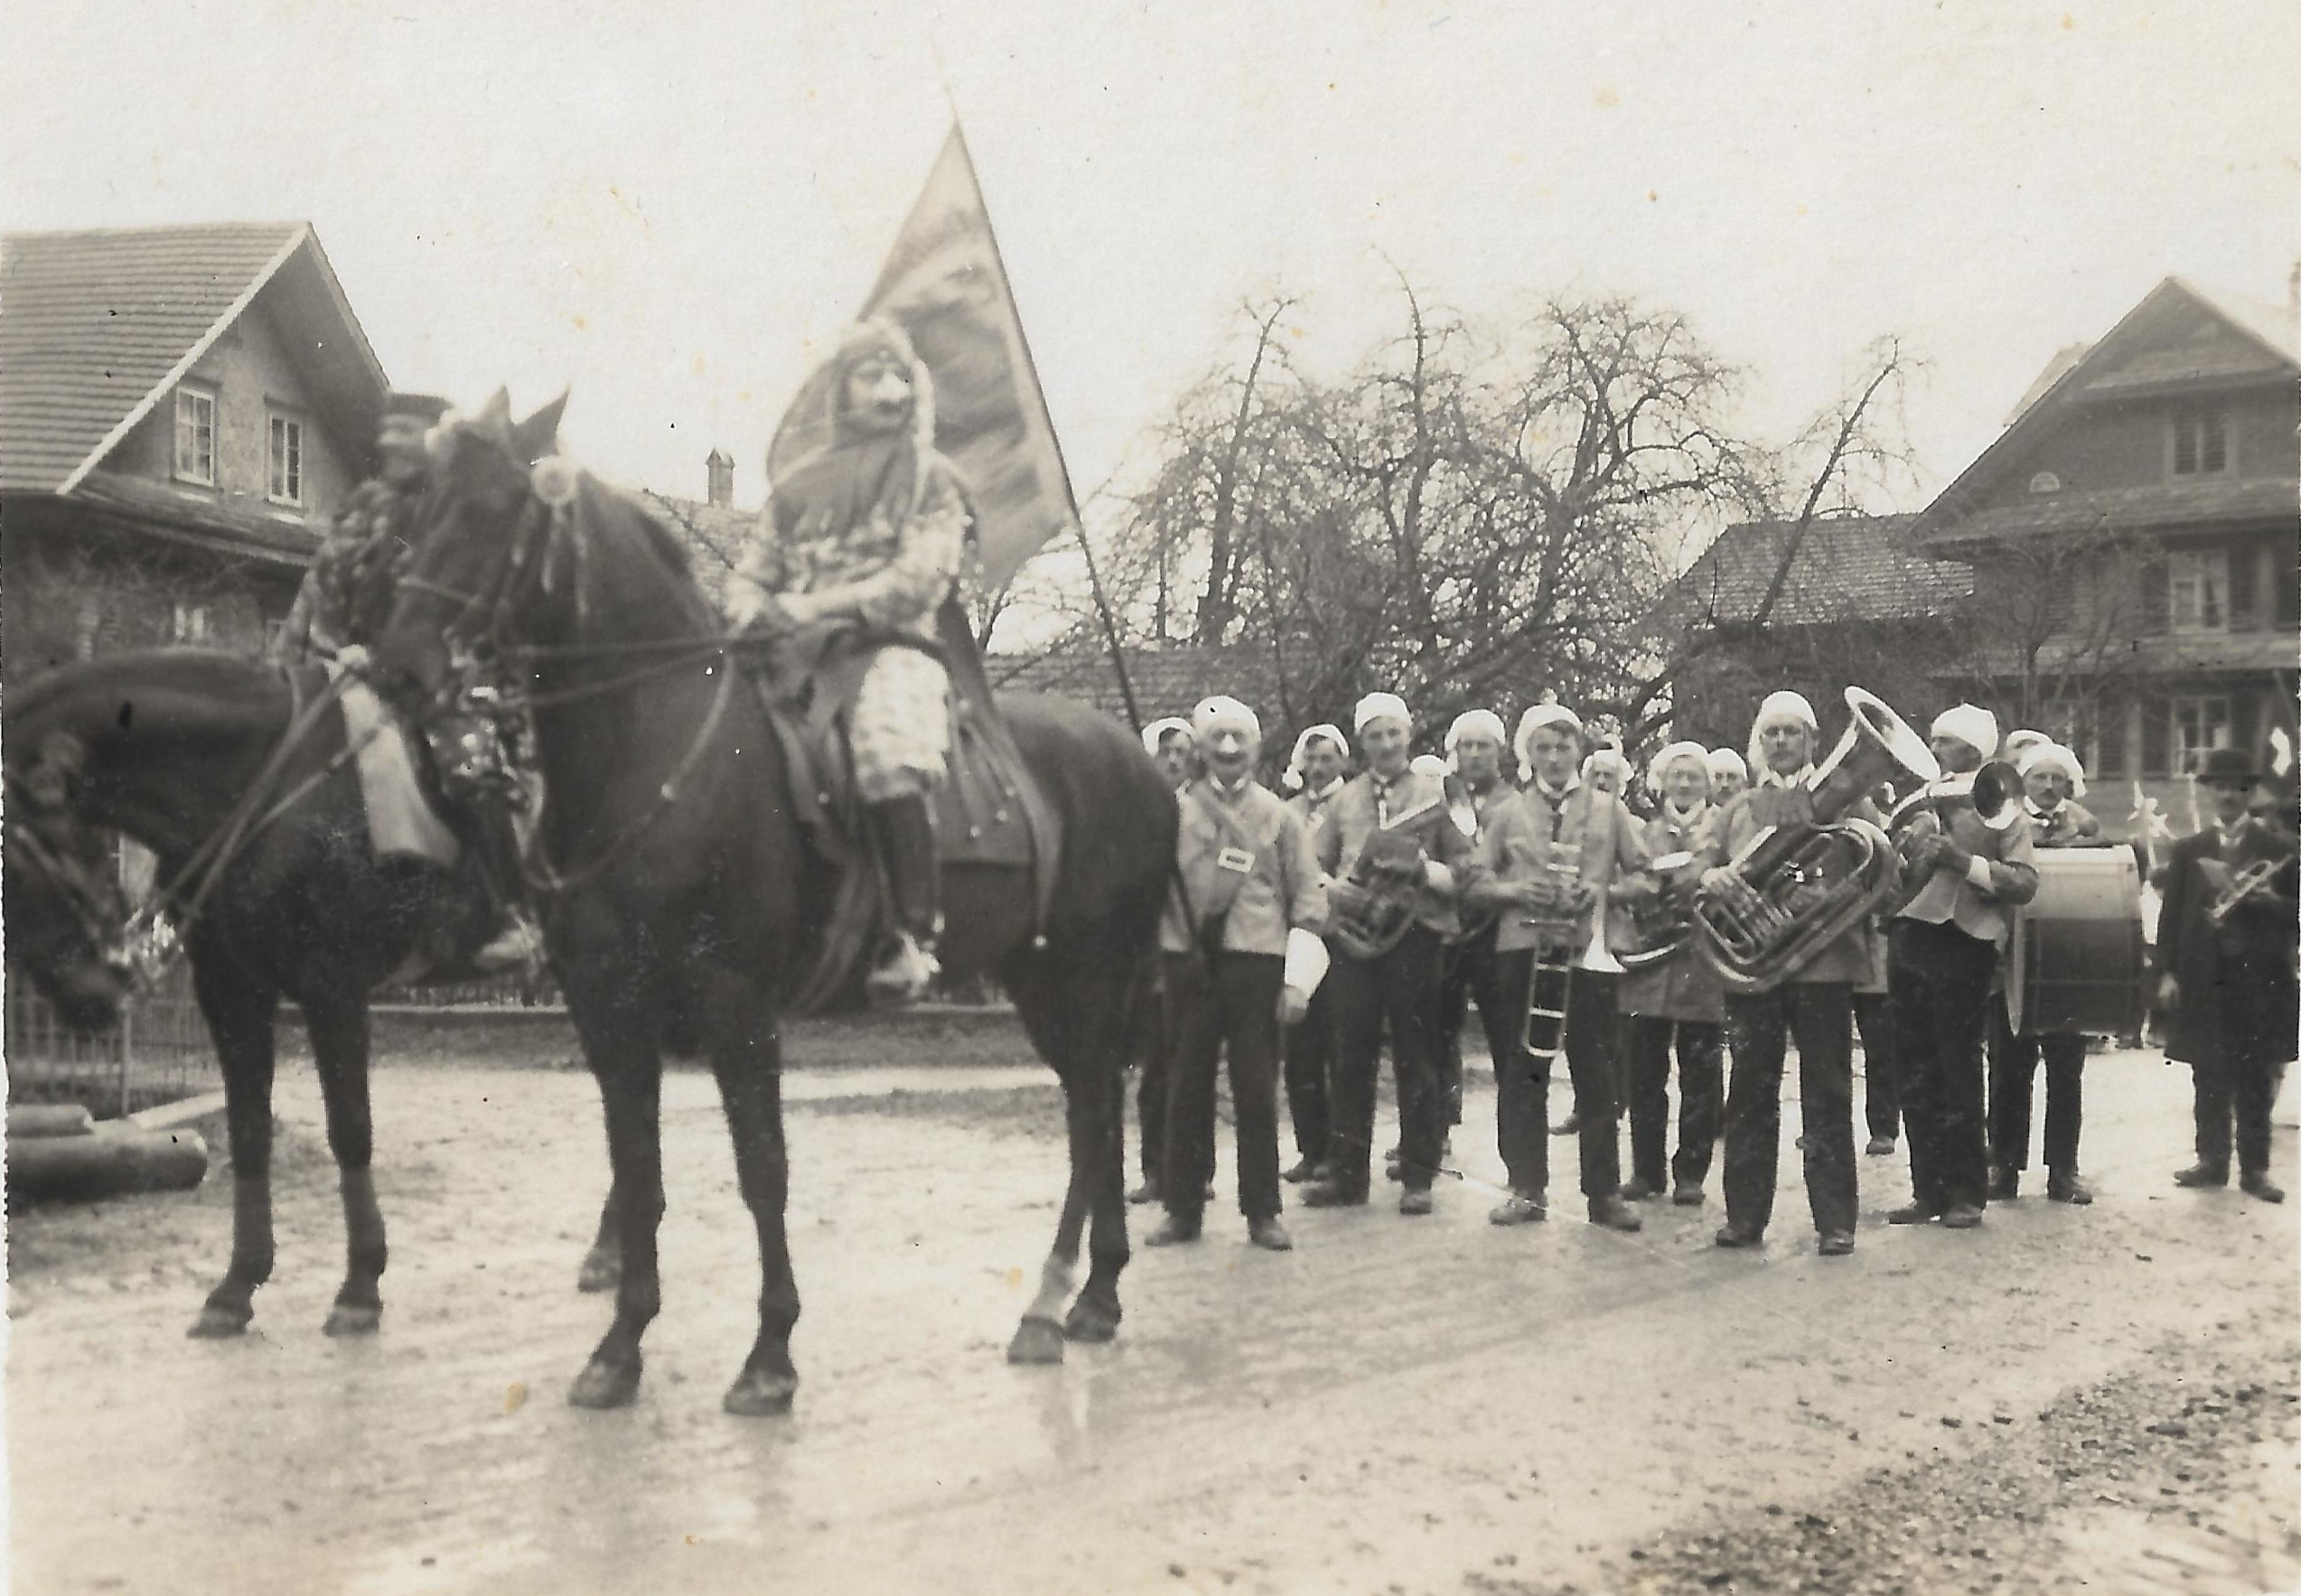
\includegraphics{./chap/1925-1950/Fasnacht-1930er.jpg}
        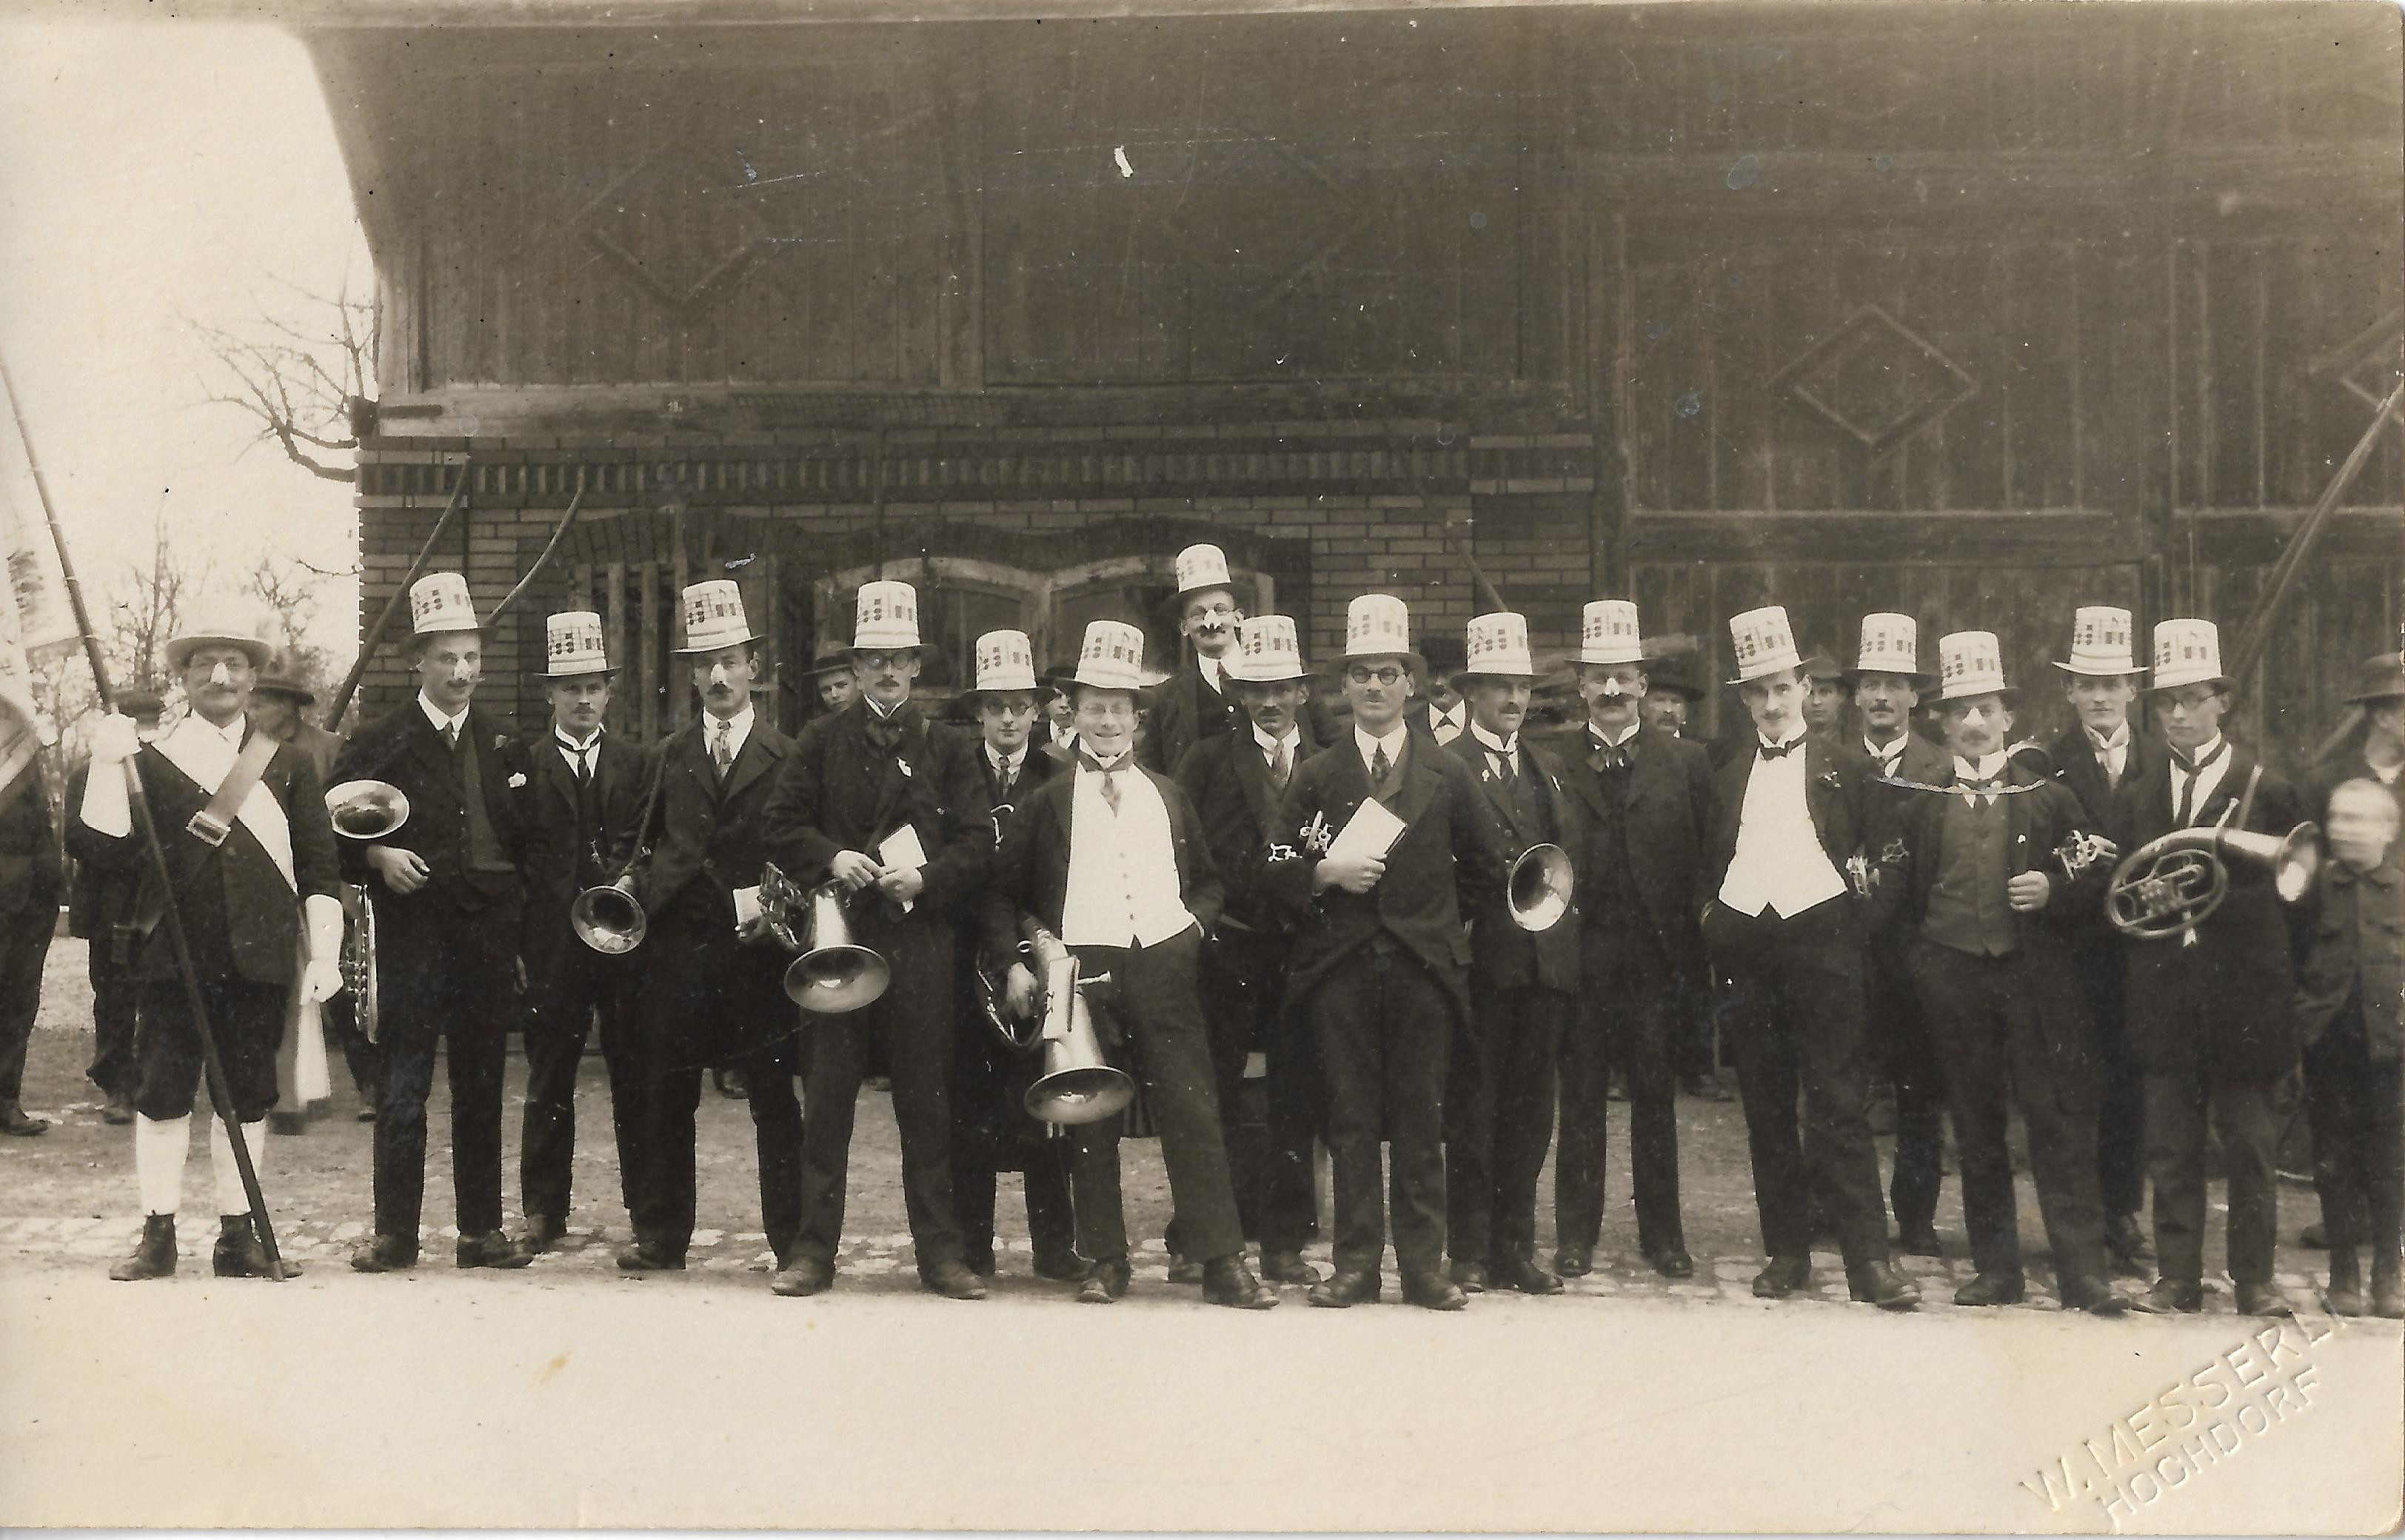
\includegraphics{./chap/1925-1950/Fasnacht-vor-Kreuz-Scheune-1930er.jpg}
    }
    \label{fig:mgh-fasnacht-1930}
    \caption{Fasnacht in den 1930ern}
\end{figure}
\begin{figure}[h]
    \centering
    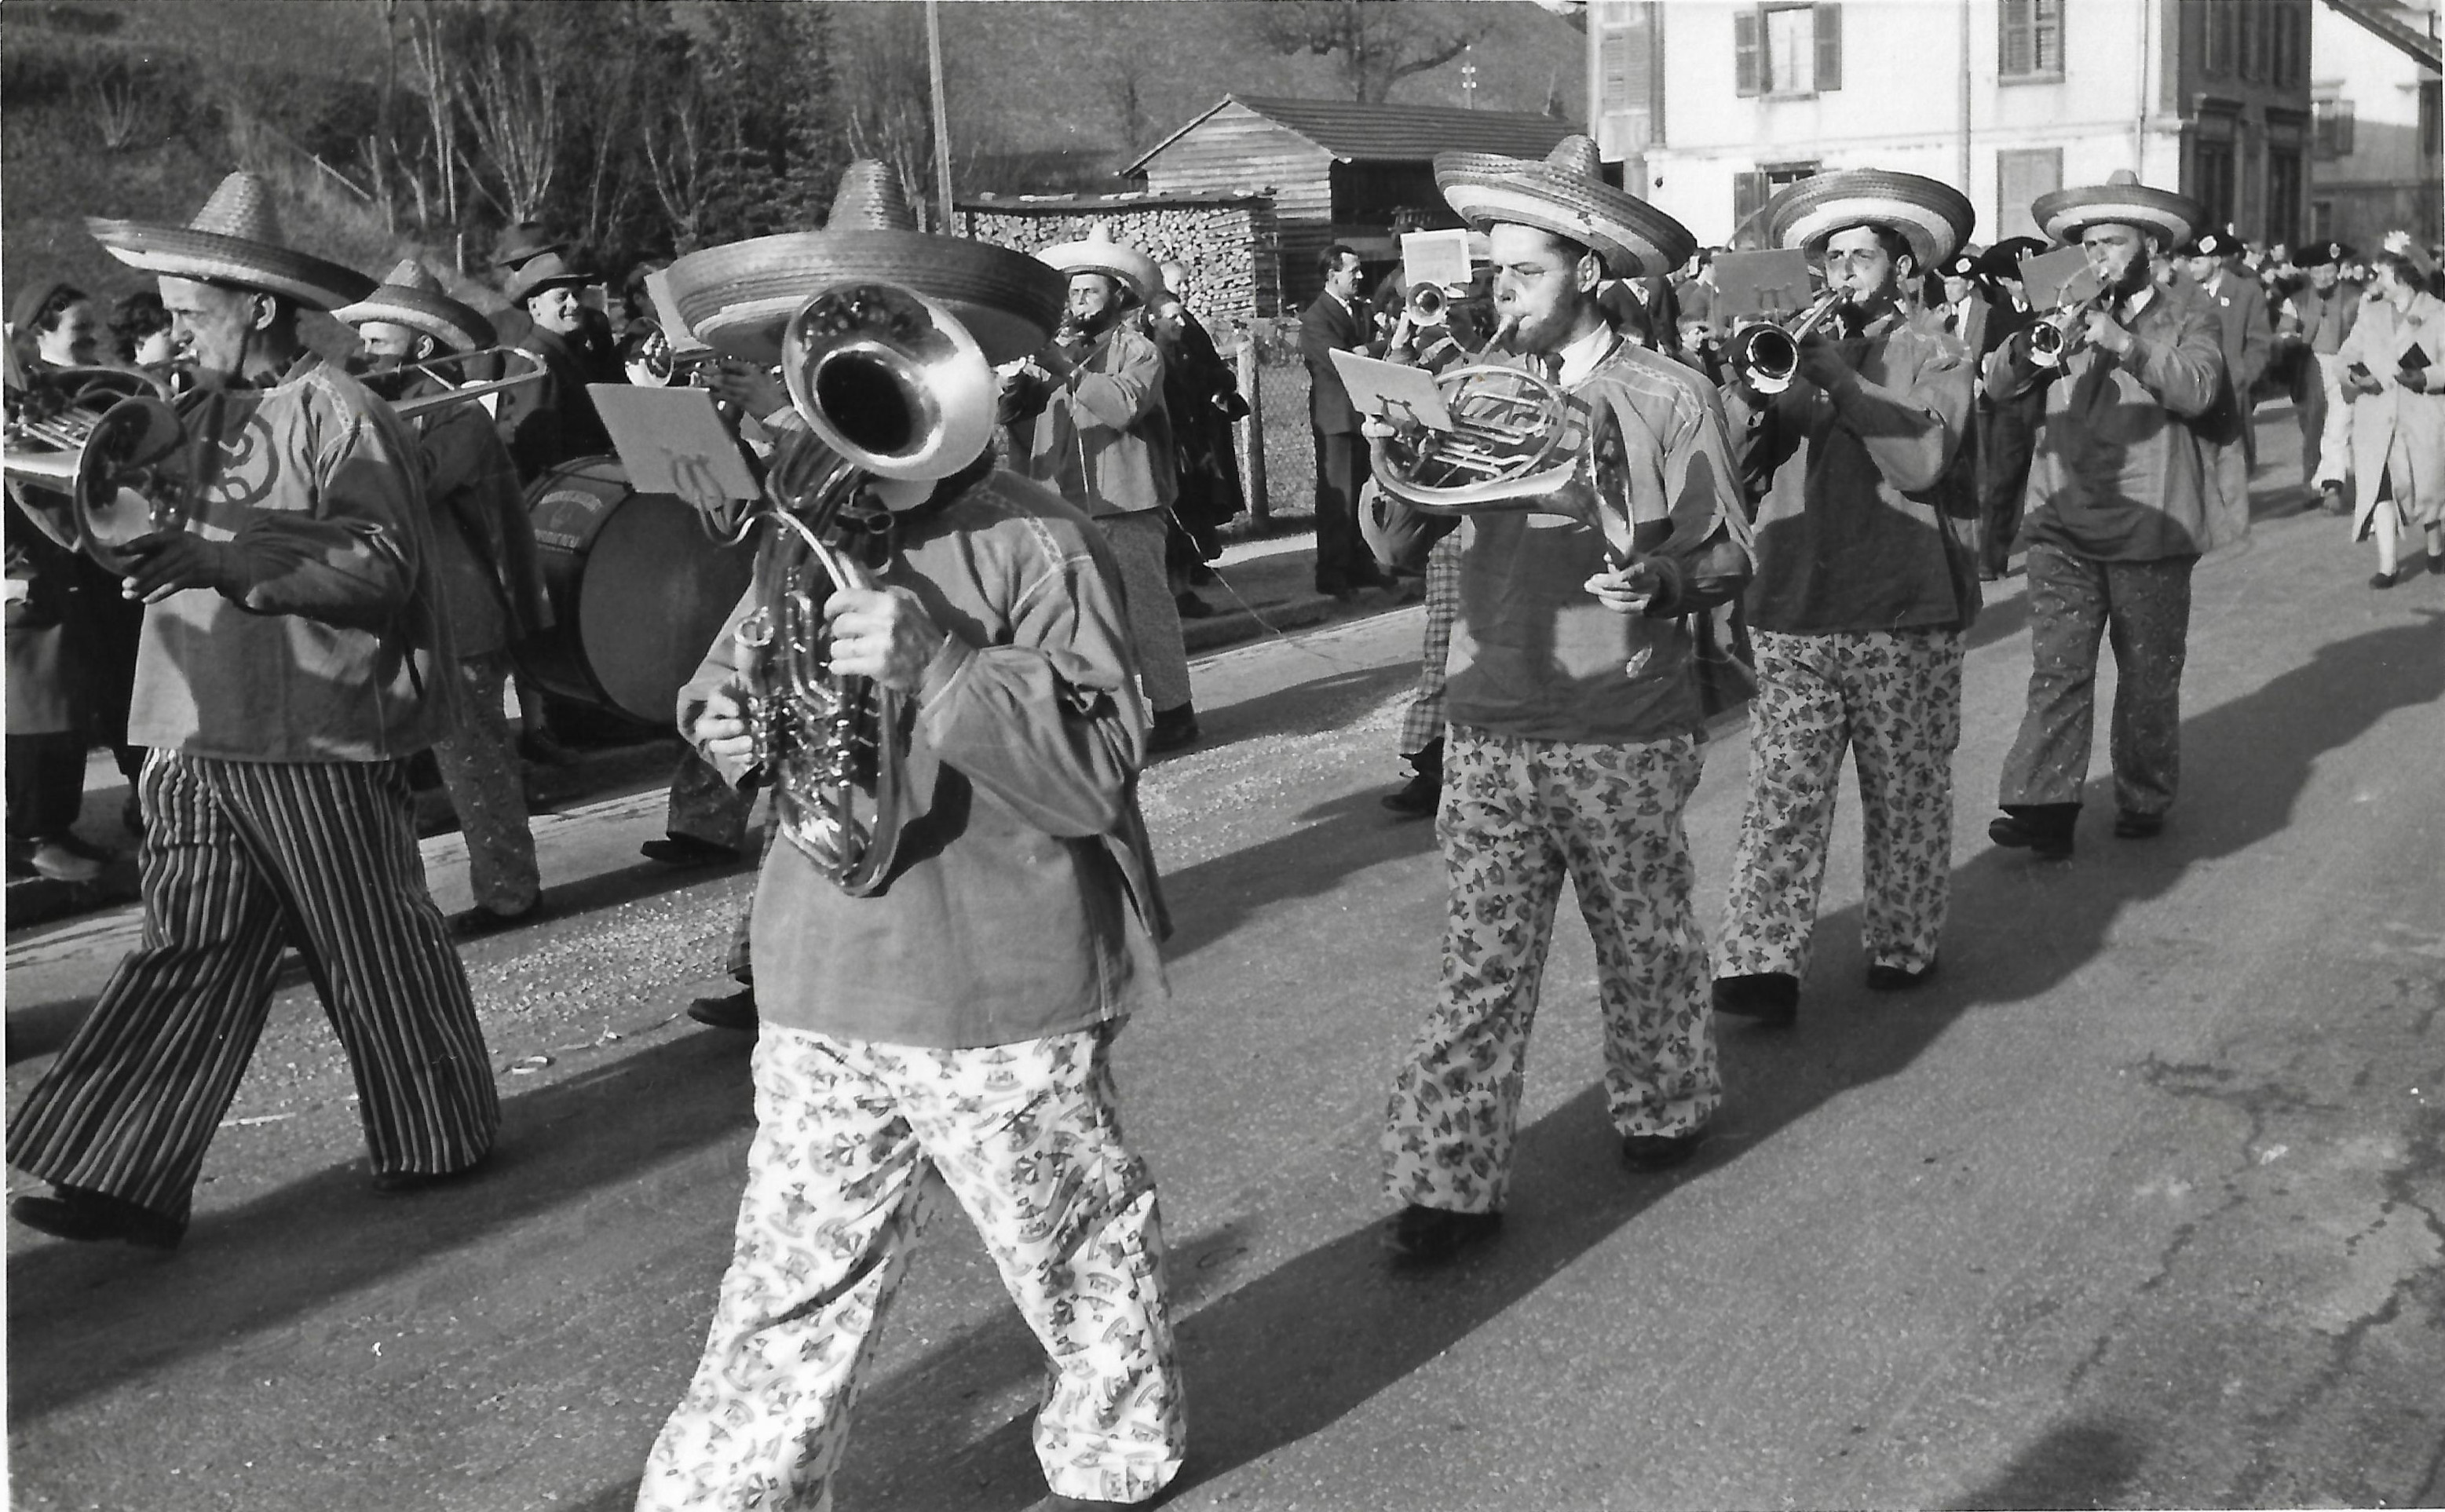
\includegraphics{./chap/1925-1950/Fasnacht-1946.jpg}
    \label{fig:mgh-fasnacht-1940}
    \caption{Fasnacht in den 1940ern}
\end{figure}
\begin{figure}[h]
    \centering
    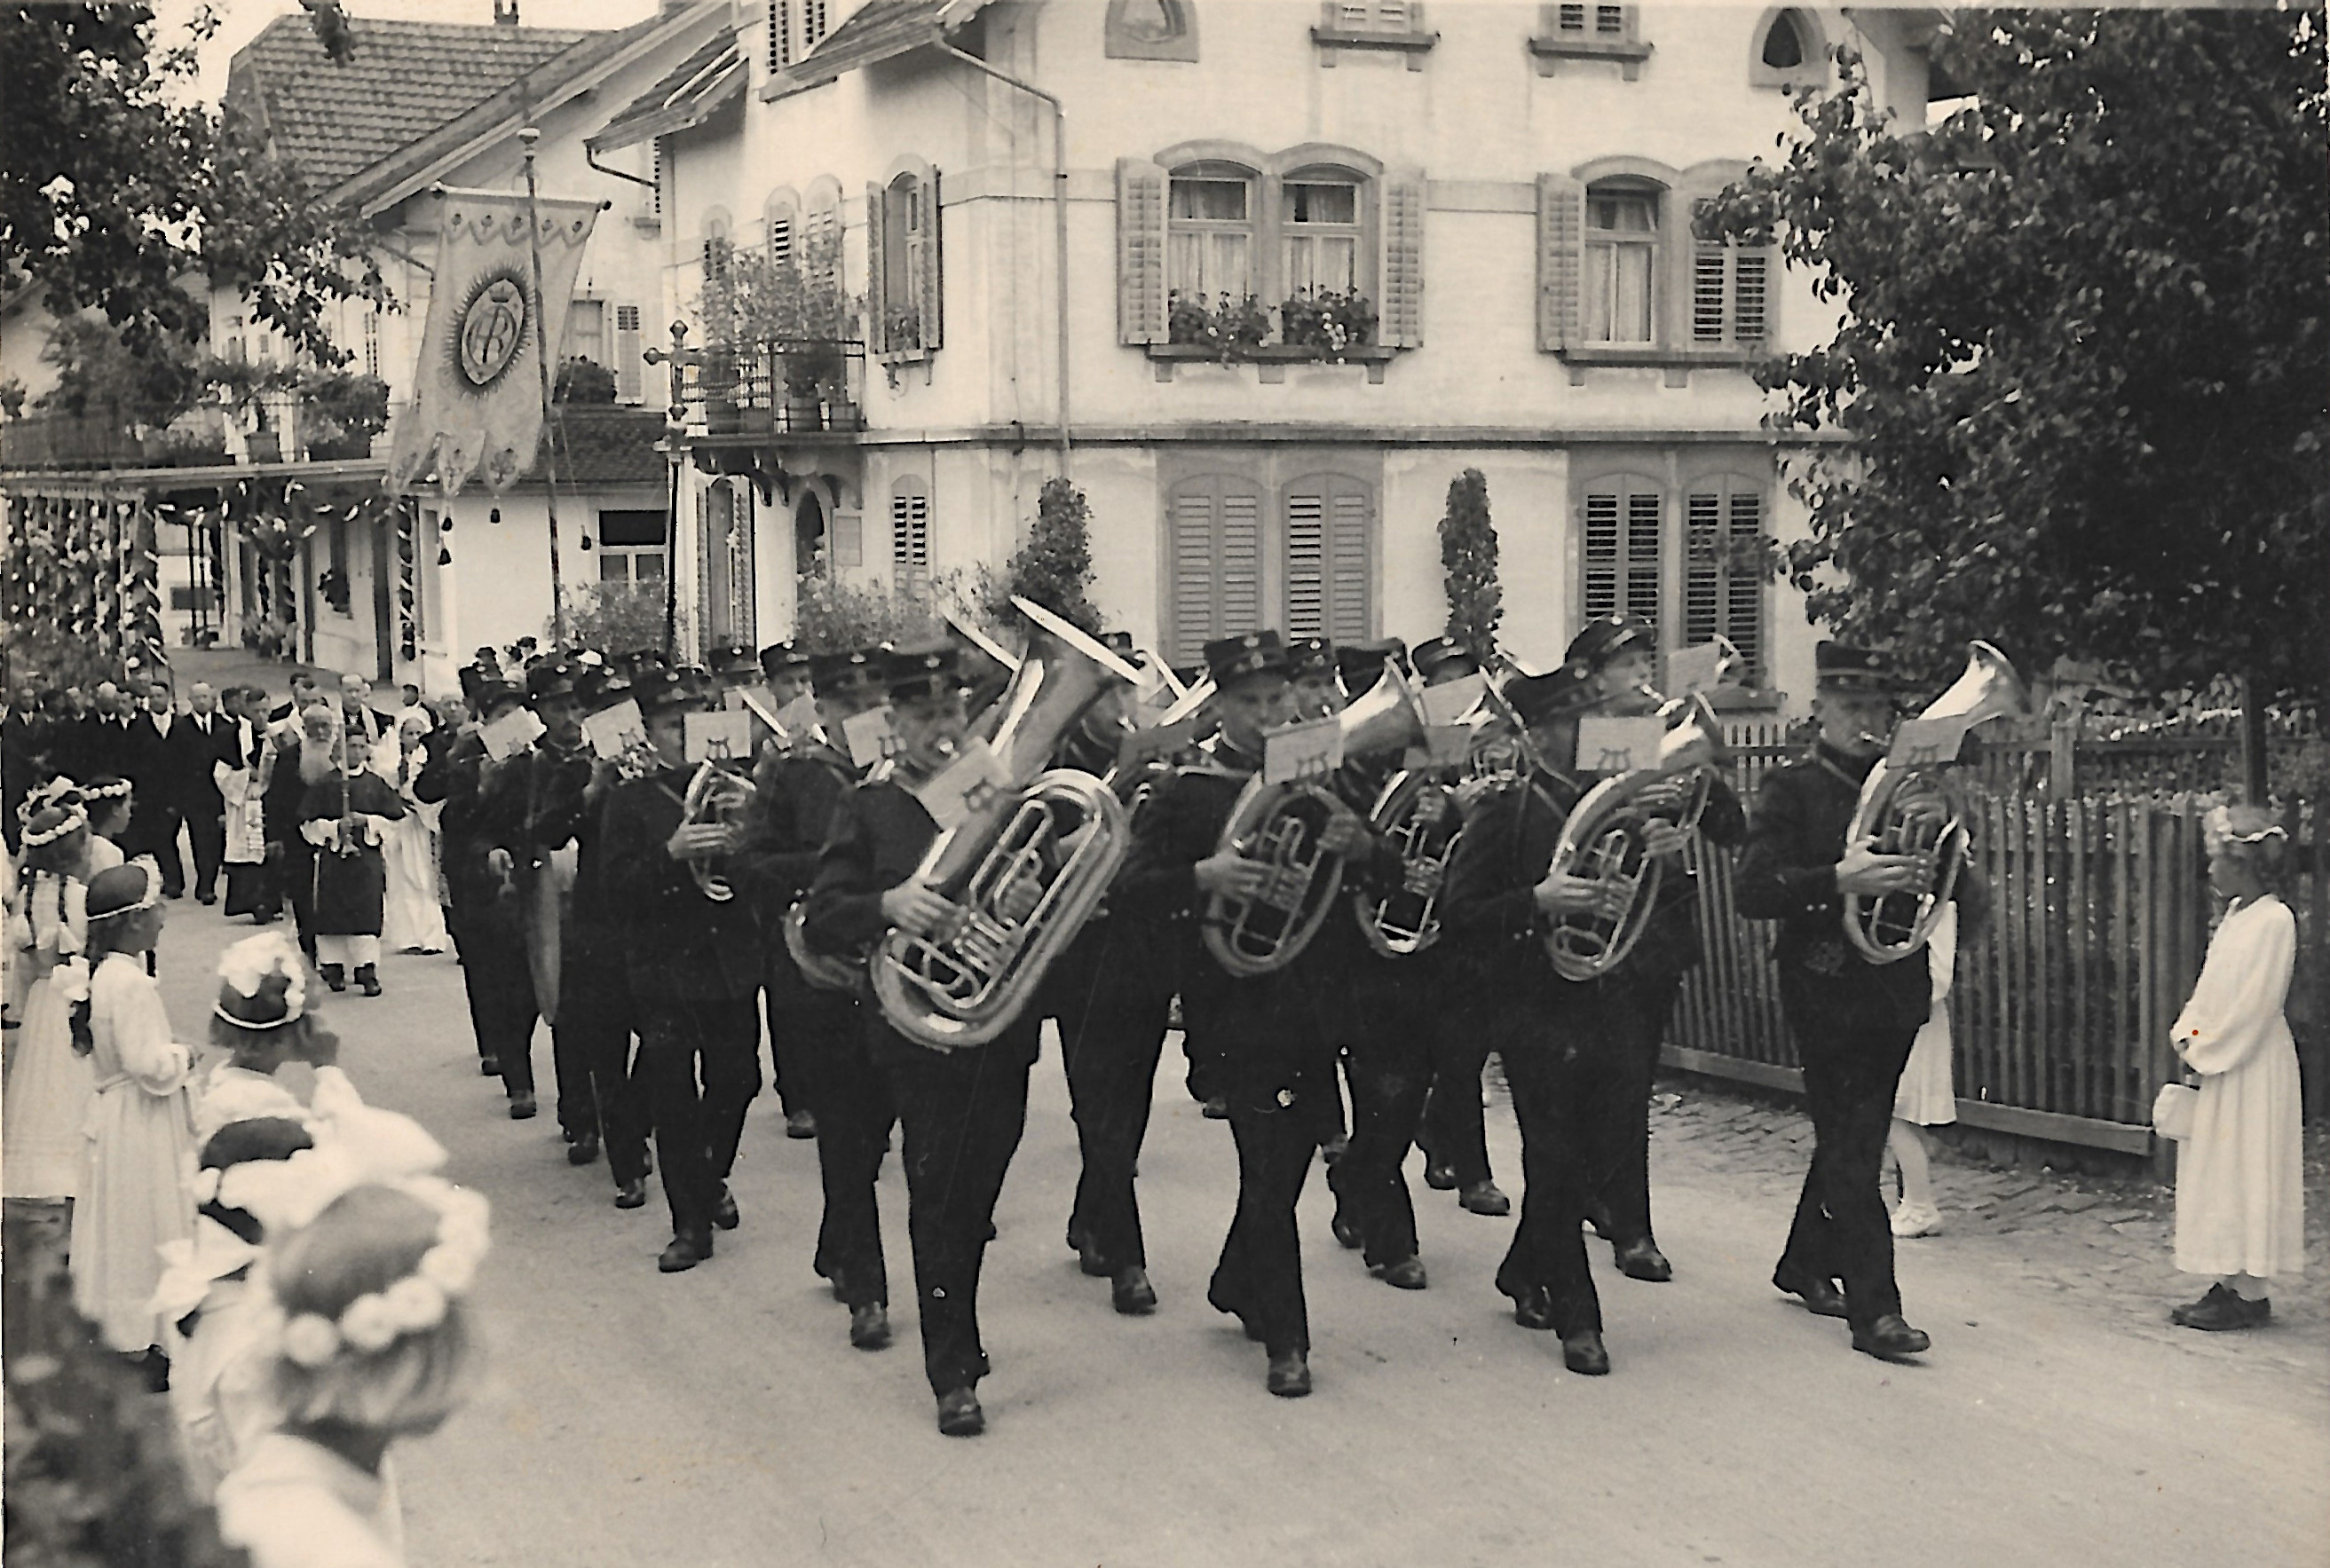
\includegraphics{./chap/1925-1950/Weisser-Sontag-1946.jpg}
    \label{fig:mgh-weisssontag-prozession}
    \caption{Weisser Sonntag 1946}
\end{figure}
\clearpage

\section{1950-1974}
\begin{figure}[p]
    \centering
    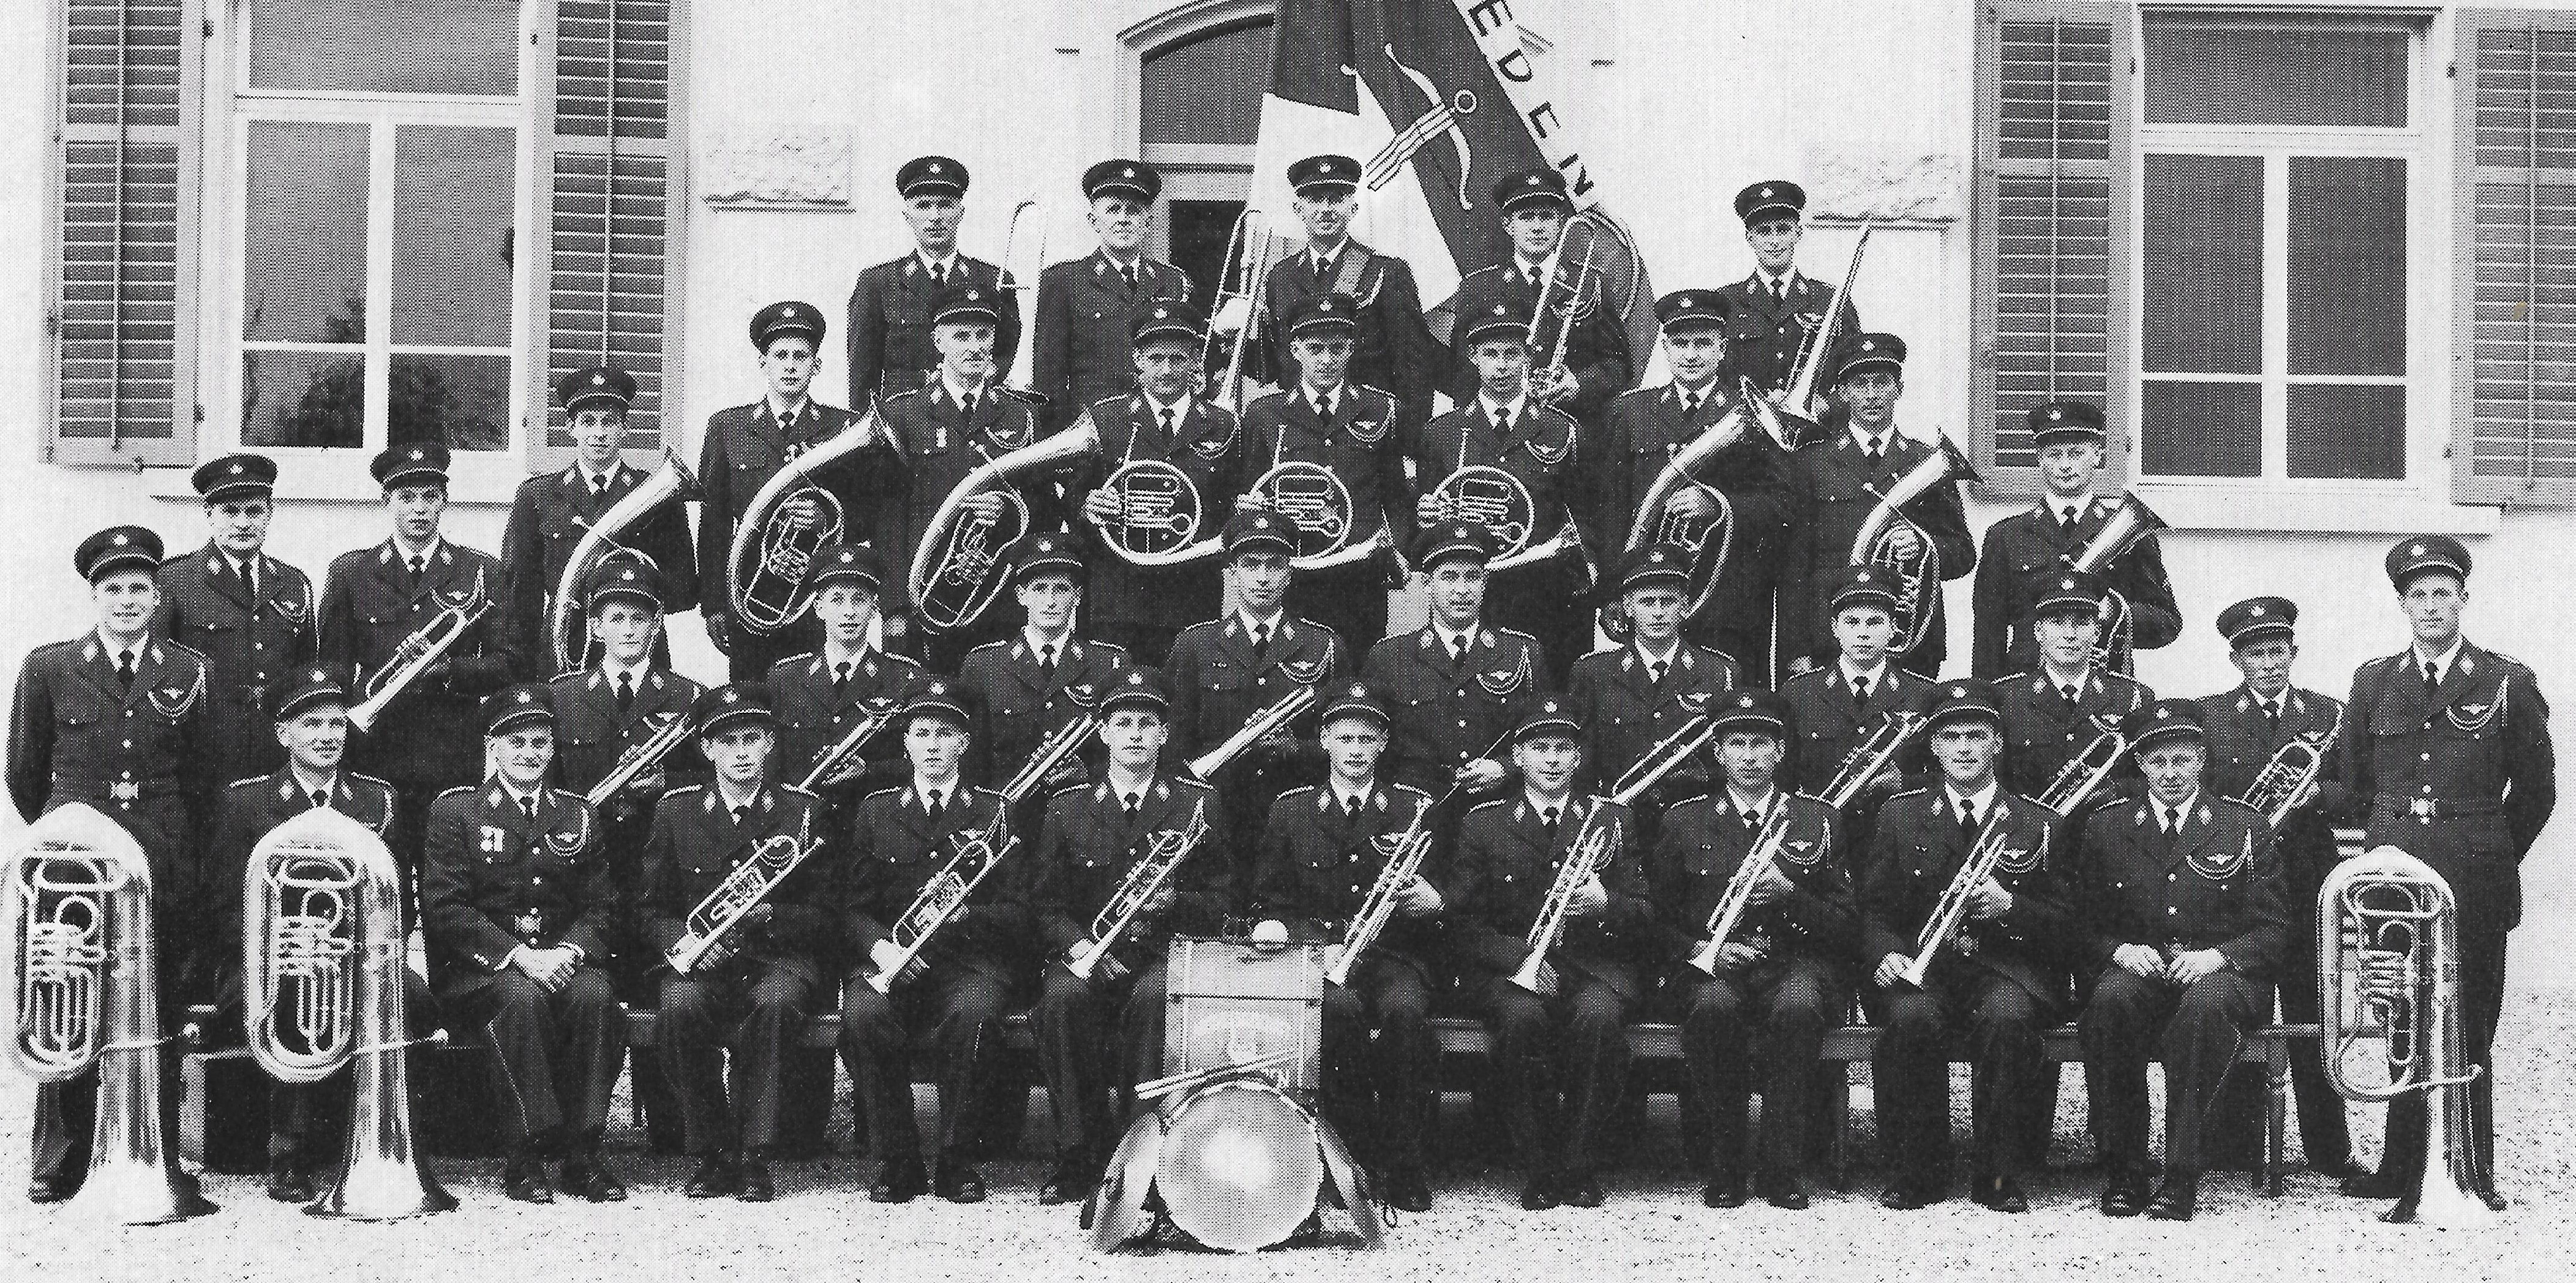
\includegraphics{./chap/1950-1974/MGH-1958.jpg}
    \label{fig:mgh-1958}
    \caption{1958}
\end{figure}
\begin{multicols}{2}

    \subsection{1950-1974}

    «Immer vorwärts», so heisst die Parole unserer Musikgesellschaft.
    Stillstand heisst Rückgang. 1955 besuchte
    man das Kantonale Musikfest in Malters und 1957
    das Eidgenössische in Zürich. Ebenso vertrat der Verein
    an den Musiktagen von Hitzkirch und Littau, sowie
    am Schwyzer Kantonal-Musikfest in Brunnen unsere
    Gemeinde. Dass Musik keine politischen Grenzen kennt,
    zeigt uns die Einladung nach Aidlingen (Stuttgart) zum
    dortigen Bezirksmusikfest

    Eine besondere Anerkennung möchten wir unseren
    Dirigenten widmen. Ihr Bestreben ist, den musikalischen
    Stand des Vereins zu heben und die Leistungen
    zu verbessern. Mit grossen Fähigkeiten und eisernem
    Willen gelang es ihnen, die Musikgesellschaft Hildisrieden
    musikalisch weiter emporzuführen. In ihren Bestrebungen
    fanden sie stets ungeteilte und geschlossene Unterstützung
    durch Vorstand und Musikanten. Wenn es trotzdem hin und wieder
    kleine Trübungen gab, so
    waren sie sicher nicht allzu ernst gemeint, denn das
    Wohl und die Ehre des Vereins standen immer im
    Vordergrund, Ihre Ratschläge, ihre grosse Aufopferung
    und Treue zur Musikgesellschaft verdient aufrichtigen
    Dank.

    Der schönste Brauch im Vereinsleben ist die Pflege des
    geselligen und kameradschaftlichen Lebens durch
    gegenseitigen Besuch. Da werden die freundschaftlichen
    Bande unter den Musikvereinen enger geknüpft. Die
    Besuche der Stadtmusik Laufen im Jahre 1952, der
    Harmonie Neuenkirch 1961, sowie jener der Aidlinger
    Blaskapelle 1972 freuten uns sehr. So werden alte,
    liebe Freundschaftsbande aufgefrischt und neue angebahnt.
    Möge dieser schöne Brauch immer erhalten
    bleiben.

    Die seit 1953 alljährlich im Hildisriederwald stattfindenden
    Waldfeste stärken die Vereinskasse (denn
    dieser Anlass wird nicht des Festes wegen organisiert).
    Dieser Anlass verursacht den Musikanten viel Mühe
    und Arbeit, ist aber bei der Bevölkerung sehr beliebt,
    wie der gute Besuch immer beweist. Die heissen
    Sommertage locken die Musikfreunde in den kühlen
    Wald, um bei Musik und Tanz einige gemütliche
    Stunden zu geniessen.

    Der 3. Juli 1954 war ein ganz besonderer Tag für die
    Musikgesellschaft, Unter dem Motto «Zoge am Boge»
    konzertierten wir in einer volkstümlichen Sendung im
    Radiostudio Basel, nebst dem Jodelklub Pilatus, Luzern,
    und dem Handharmonika-Duett Lustenberger, Emmenbrücke.
    Der schöne Erfolg gab dem Verein den nötigen
    Impuls für die Weiterreise nach Laufen zur dortigen
    Stadtmusik, um an der Jubiläumsfeier teilzunehmen.
    Die Feierlichkeiten eröffneten die Musikgesellschaft
    Konkordia Allschwil, der Männerchor Laufen und
    schliesslich die Hildisrieder Musikanten. Die musikalischen Darbietungen,
    sowie die humoristischen Einlagen von Mathias Jutz als Conferencier ernteten
    rauschenden Beifall. Im September gleichen Jahres
    durften wir die Grenzbesetzungssoldaten der Mitr Kp. 4
    mit einem Konzert erfreuen

    Trotz Schneegestöber am Auffahrtsmorgen vom
    19. Mai 1955, wurde dann der Abend zu einer sehr
    eindrucksvollen Feier. Der Empfang zu Ehren des neu
    gewählten Regierungsrates Dr. Werner Bühlmann
    war ein einmaliges Erlebnis

    Die Musikgesellschaft ist 1955 auf 31 Mitglieder angewachsen, und der Vorstand setzte sich wie folgt
    zusammen:

    Präsident: Hans Troxler, Ausserbuchen
    Aktuar: Kaspar Troxler, Moos
    Kassier: Josef Rüttimann, Dorf
    Mat.-Verwalter: Otto Estermann, Traselingen
    Beisitzer: Hans Suppiger, Dorf

    1956 wirkte unser Verein an der Luzerner-Fasnacht
    mit. Die Musikanten waren als Zahnärzte verkleidet.
    Der zahlenmässig erstarkte Verein stand 1957 vor der
    Wahl einer neuen Uniform. Mit tatkräftiger Unterstützung seitens der vielen
    Gönner konnte die Neuuniformierung beschlossen werden.

    Mit dem neuen Kleid zogen unsere Musikanten
    erstmals an das eidgenössische Musikfest in
    Zürich. Neben vielen Proben und Auftritten gehört
    hin und wieder eine verdiente, gemütliche Reise ins
    Programm, um die Kameradschaft zu beleben. Wir
    erinnern an die Ausflüge an den Rheinfall 1950, ins
    Bündnerland 1952, ins Tessin 1956, auf die Rigi 1958,
    ins Urnerland 1960, ins Lötschental 1962, auf die
    Schwägalp 1964, in das Engadin 1967, die Drei-See-Rundfahrt 1969 und die Reise auf die Rieder- und
    Bettmeralp 1972.

    Da viele Musikanten zu den besten Schützen unserer
    Gemeinde zählen, ist es für die Musikgesellschaft stets
    eine Freude, diese bei der Heimkehr von grossen
    Schützenfesten feierlich zu empfangen. Am Freundschaftstreffen 1961 mit der Harmonie Neuenkirch
    in Neuenkirch übergab Präsident Silvester Troxler
    seinen Musikfreunden die Ehrenurkunde.

    Am 24. Februar 1962 konzertierten unsere Musikanten
    zur Eröffnung des neuerbauten Gasthof zum Roten
    Löwen und ebenso im November zum Antrinket im
    renovierten Restaurant Kreuz.

    Der 29. November 1962 war ein denkwürdiger Tag für
    unser Dorf, Regierungsrat Franz Xaver Leu übergab
    die neue Dorfstrasse dem Verkehr. Dem Dorfausbau
    mussten neun Häuser weichen. Der "`Vierwaldstätterhof"', als`grösstes Verkehrshindernis, war lange Zeit
    ein dankbares Fasnacht-Sujet, das allerdings schon
    Jahre vorher vom unvergesslichen Mathis Jutz mehrmals
    entrümpelt wurde.

    Die Generalversammlung vom 12. März 1966 beschloss
    die Neuanschaffung von Instrumenten. Man kaufte
    7 Flügelhörner & Fr. 580.—, 2 Euphonium zu Franken
    1350.—, 1 Es-Bass & Fr. 2200,— der Marke Wilson
    von Kurath, Flums, sowie 5 Courtois-Trompeten A
    Fr. 530.—.

    Im Sommer 1970 erlebten die Hildisrieder einen Pfarr-
    auftritt, Dekan Josef Jost von Beromünster, vorher
    Pfarrer in Hochdorf wurde Pfarrherr von Hildisrieden.
    An der Delegiertenversammlung des Kantonalen
    Musikverbandes 1972 in Kriens wurde der Musiktag
    Hildisrieden übertragen.

    Kann man sich ein Fest denken ohne Musik? Nach
    meiner Auffassung sicher nicht. Wo immer die Klänge
    einer Musik ertönen, herrscht froher Sinn und Gemütlichkeit.
    Wohin auch die Musikgesellschaft Hildisrieden gerufen wird, ist sie bereit, mitzumachen.
    Mit besonderer Freude folgt sie jeweils den Einladungen
    von Nachbarsektionen zu einer Banner- oder Uniformweihe.

    Die Stadtmusik Laufen, mit der sie freundschaftliche
    Beziehungen pflegt, rief sie zu einem Gala-Konzert.
    Ein Kurplatzkonzert in Luzern zu geben und mit
    ihren Darbietungen Gäste aus aller Welt zu erfreuen,
    zählt zu ihren dankbaren Ereignissen. Die Hildisrieder-Fasnacht beleben und der Götschizunft eine
    Freude zu bereiten beweist, dass sie auch Verständnis
    für echtes Brauchtum hat. Auch andere Feste verschönern, gehört zu ihrer Aufgabe. Mit den Vereinen
    von Hildisrieden begeht sie nach vollendetem Tagewerk
    den 1. August.

    So oft der hochwürdige Bischof zur Firmung unsere
    Gemeinde besuchte, oder ein Pfarrer oder Primiziant
    Einzug hielt, fehlte auch das zu ihren Ehren gegebene
    Ständchen auf dem Dorfplatz nicht.

    Ein schöner Brauch, den der Verein pflegt, ist, den
    neuvermählten Kameraden ein Ständchen zu bringen.
    Die gleiche Aufmerksamkeit wird auch den verehrten
    Jubilaren anlässlich des Geburtstages oder der Goldenen
    Hochzeit zuteil. Oft schon stand die Musikgesellschaft
    am Grabe eines lieben Aktiv- oder Ehrenmitgliedes.
    Wehmutsvoll senkte sich jeweils das Vereinsbanner
    unter den Klängen des letzten Musikgrusses in die kühle
    Gruft. Auch die grösseren und kleineren Ausmärsche
    in die nähere Umgebung, die speziell unseren Gönnern
    und Freunden gewidmet sind, und die sich zur Ausbildung in der Marschmusik eignen, seien hier erwähnt.
    Wir schön, dass die Musikgesellschaft nach dem Motto
    handelt: «In Freud und Leid, zum Spiel bereit.»


\end{multicols}

\begin{figure}[h]
    \centering
    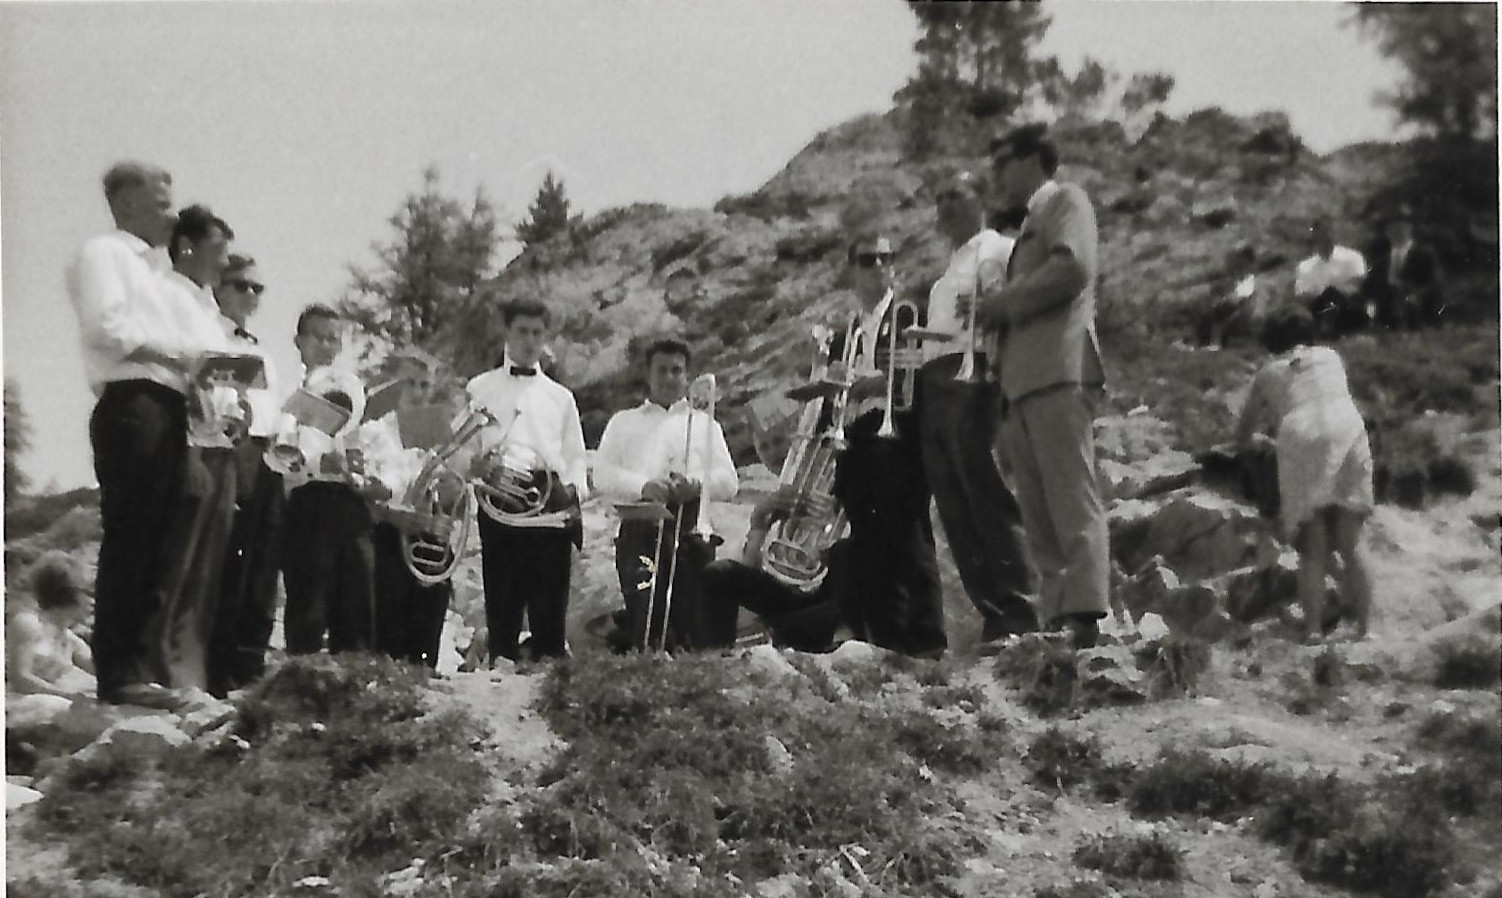
\includegraphics[scale=2.0]{./chap/1950-1974/Musikreise-1960er.jpg}
    \label{fig:mgh-musigreise-1960}
    \caption{Musikreise 1960}
\end{figure}


\chapter{1974-1999}

\newcounter{year}
\forloop{year}{1974}{\value{year} < 2000}%
{%
    \section{\arabic{year}}
    \begin{figure}[p]
        \centerline{\includegraphics[max
        size={\textwidth}{\textheight},keepaspectratio]{./chap/1974-1999/\arabic{year}/\arabic{year}.pdf}}
    \end{figure}
    \input{./chap/1974-1999/\arabic{year}/Jahresbericht.tex}
    \clearpage
}

\chapter{2000-2024}
\forloop{year}{2000}{\value{year} < 2024}%
{%
    \section{\arabic{year}} \ifnum\value{year}=2021
    \else
    \begin{figure}[p]
        \centerline{\includegraphics[max
        size={\textwidth}{\textheight},keepaspectratio]{./chap/2000-2024/\arabic{year}/\arabic{year}.pdf}}
    \end{figure}
    \fi
    \input{./chap/2000-2024/\arabic{year}/Jahresbericht.tex}
    \clearpage
}

\end{document}